% !TEX root = main.tex

% TODO:
% REMARK:

\section{CP Asymmetry in Top quarks pair and corresponding observables/models}
\label{sec:AcpModelObs}

	With the real 2016 data from CMS, a complete analysis on $t\bar{t}$ CPV is done and mentioned in previous chapters. The analysis focuses on the CPV probable coming from the $t\bar{t}$ in CEDM model and it uses the triple products to be the CP observable to do the measurement on the data. However, there are not only triple products' type observable could be used, but also another type which is characterized as T-even observables; There are also not only CEDM model could be the source of top quarks' CPV, but 2HDM model which has been discussed since decades. 

	\subsection{Models}
	\label{ssec:AcpModel}

		In reference \cite{Atwood:2000tu}, it is particularly organized the information about CPV in top quarks. The usual discussions about CPV in top quarks are related to CEDM model and 2HDM model.

		\subsubsection{ CEDM model}
		\label{sssec:AcpModel_CEDM}



			The CEDM model's asymmtry from real part of $d_t^g$ could be detected by T-odd observables only, and imagininary part of $d_t^g$ could be detected by T-even observables.(T-odd and T-even will be menntioned in section\ref{ssec:AcpObs}) However, the implementation to generate the model lagrangian with program FeynRules(cite****), the imaginary part of $d_t^g$ is not allowed inputting. Now, therefore, the MadGraph generator we use could not make CEDM sample with imaginary part of $d_t^g$. If there will be hacked into the FeynRules and successfully imsert the restricted imaginary part now, the T-even observable behavior corresponding to $Im(d_t^g)$ will be still an interesting issue.

		\subsubsection{ 2HDM model}
		\label{sssec:AcpModel_2HDM}

			The only detected neural Higgs-boson in standard model is CP and flavor conserving automatically. However, the extended Higgs sector could be allowed feature of  CP violation. The beyond standard model's 2HDM model is the probable case and one of simple case of Higgs sector with CP violation. For the top quark, because of it's heavy mass, the larger effect of CPV is expected in the Higgs sector. It is known that 2hDM extensions with natural flavour conservation at the tree level and explicit CP violation are by complex Yukawa coupling matrices which lead to a Kobayashi-Maskawa (KM) phase, and also by tree level Higgs potential V($\Phi_1$, $\Phi_2$). CP violation in the scalar potential induces blending of CP–even and –odd scalars, and in this way leading to 3 mass eigenstates but not CP eigenstates, so we have couplings:

			\begin{equation}
			\begin{split}
			L_Y = -(\sqrt{2} G_F)^{1/2}\sum_{j,f}^{}m_f(a_{jf}\bar{f}f + \~{a}_{jf} \bar{f} i \gamma_5 f)\phi_j
			\label{eq:2HDM_scalar}
			\end{split}
			\end{equation}
			\FloatBarrier

			where the $G_F$ is Fermi’s constant, f presents a quark/lepton field and $m_f$ its associated mass, and $a_{jf}$ , $\~{a}_{jf}$ are the reduced (pseudo)scalar Yukawa couplings. The couplings are related to parameters of the scalar potential. And for the top quark:

			\begin{equation}
			\begin{split}
			L_Y = -(\sqrt{2} G_F)^{1/2}\sum_{j=1}^{3}m_t(a_{jt}\bar{t}t + \~{a}_{jt} \bar{f} i \gamma_5 t)\phi_j \;\;\;\;\;\;\;\;\;\;\;\;\;\;\;\;\\
			a_{jt} = d_{2j}/\sin{\beta} \; \; , \; \; \; \; \; \~{a}_{jt} = -d_{3j}\cot{\beta} \; \; , \; \; \; \; \; \tan{\beta} = v_2/v_1
			\label{eq:2HDM_scalar_t}
			\end{split}
			\end{equation}
			\FloatBarrier

			$v_1$, $v_2$ are the vacuum expectation values of the two doublets, and $d_{2j}$, $d_{3j}$ are the matrix elements of a 3×3 orthogonal matrix which describes the mixing of the neutral states. To do the measurement of CPV in flavor–diagonal reactions like $gg \rightarrow t\bar{t}$, $qq^- \rightarrow t\bar{t}$ is:

			\begin{equation}
			\begin{split}
			\gamma_{cp} = -a \widetilde{a} = d_{2j}d_{3j}\cot{\beta}/\sin{\beta}
			\label{eq:2HDM_rawCPV}
			\end{split}
			\end{equation}
			\FloatBarrier

			Futhermore, the CP violation in the Higgs sector can be evoked in the model where the coupling in the Higgs potential is complex. The complex coupling may cause the CP-violating interaction directly, and the complex VEV(vacuum expectation value)'s of of Higgs field that could contain CPV effect. Also, the real potential could lead to a ground state in which CP breaks spontaneously. The tree-level Higgs potential of 2HDM model is shown below:(Eq.\ref{eq:2HDM_potential})

			\begin{equation}
			\begin{split}
			V(\Phi_1, \Phi_2) = -\mu^2_{11} \Phi^{\dagger}_{1}\Phi_{1} -\mu^2_{22} \Phi^{\dagger}_{2}\Phi_{2} - ( \mu^2_{12} \Phi^{\dagger}_{1}\Phi_{2} + h.c.) \\
			+ \lambda_1(\Phi^{\dagger}_{1}\Phi_{1})^2 + \lambda_2(\Phi^{\dagger}_{2}\Phi_{2})^2 + \lambda_3(\Phi^{\dagger}_{1}\Phi_{1}\Phi^{\dagger}_{2}\Phi_{2}) + \lambda_4(\Phi^{\dagger}_{1}\Phi_{2})(\Phi^{\dagger}_{2}\Phi_{1})\\
			+ \frac{1}{2}[\lambda_5(\Phi^{\dagger}_{1}\Phi_{2})^2 + h.c. ] + [ \lambda_6 \Phi^{\dagger}_{1}\Phi_{1}\Phi^{\dagger}_{1}\Phi_{2} + \lambda_7 \Phi^{\dagger}_{2}\Phi_{2}\Phi^{\dagger}_{2}\Phi_{1} + h.c.]
			\label{eq:2HDM_potential}
			\end{split}
			\end{equation}
			\FloatBarrier

			The particle spectrum of 2HDM model are three neutral Higgs-bosons and 2 charged Higgs-bosons which are denoted by $H^{k}$(k=1,2,3) and $H^{+(-)}$. The key parameters of 2HDM model which could lead to CP violation in the Higgs sector are $\lambda_5$, $\lambda_6$, $\lambda_7$, and $\mu_{12}^2$, and there are some organized scenario could be found from \cite{Atwood:2000tu}.

			The previous organization and more 2HDM model and parameters discussion would be in the refernce of particle-phenomenology papers \cite{Atwood:2000tu}, \cite{ElKaffas:2006gdt}, \cite{Khater:2003wq}, \cite{Keus:2015hva}, \cite{Iguro:2019zlc}, \cite{Bernreuther:1993hq}, \cite{Bernreuther:1998qv}. 

			2HDM model's CPV could be detected by CP-odd observables with both T-odd or T-even property according to the derivation (ref 1993derivation). Because the parameters in 2HDM model is too comlicated to tune, it is not the bottom line of us to approach. Some research of parameter setting related to CPV in top quarks would be approached in citation at last paragraph. Therefore, there will be done by some fundamental test of default parameter setting in the section.\ref{ssec:AcpObs} with various observables.



	\subsection{Observables}
	\label{ssec:AcpObs}

		The probed observables are roughly classified to two type. The first one is the CP-odd observables which is T-odd and the other is CP-odd observable which is T-even. The even/odd means the $\hat{CP}$/$\hat{T}$ operator's eigenstate with eigenvalue $+1$/$-1$. The triple product type observable(for example, the $O_{3,6,12,14}$ we use in the 2016 analysis) is T-odd observable. The introduction of T-odd CP-odd observable is mentioned in section***** before, and the T-odd observables of CPV is maturely developed and extensively used, so I will put emphasis on T-even observables in this section, and just make a simple test to T-odd observables in following contents.

		\subsubsection{Classification and Test}
		\label{sssec:AcpObs_class_test}

			The following testing are based on some simulation sample of $t\bar{t}$ by generator Madgraph to generate parton-level's event-by-event sample. And the showering and detector simulation would be done by Pythia cite**** and Delphes cite****.

			At first, following the paper\cite{Hayreter:2015ryk}'s(which is the basic of 2016 analysis) selection and model implementation, we also use Madgraph\cite{Alwall:2011uj} generator as it to generate $t\bar{t}$ sample of CEDM model to double-check the triple product observables action under CEDM model. There are generated samples at $d_t^g$ tuning to be 0 to 5.0 to see the relation between $A_{cp}$ and parameter $d_t^g$. The $O_{3}$, $O_{6}$, $O_{12}$, $O_{14}$ would be tested:

			\begin{figure}[H]
			\centering
			    \subfigure[$O_{3}$]{\includegraphics[width=0.45\textwidth]{Figures/Observables/O_{3}.pdf}}
			    \subfigure[$O_{6}$]{\includegraphics[width=0.45\textwidth]{Figures/Observables/O_{6}.pdf}}\\
			\end{figure}
			\FloatBarrier
			\begin{figure}[H]
			\centering
			    \subfigure[$O_{12}$]{\includegraphics[width=0.45\textwidth]{Figures/Observables/O_{12}.pdf}}
			    \subfigure[$O_{14}$]{\includegraphics[width=0.45\textwidth]{Figures/Observables/O_{14}.pdf}}\\
			\caption{Reproduction of the results from \cite{Hayreter:2015ryk}}
			\label{Obs:fig:reproduce}
			\end{figure}
			\FloatBarrier


			Also, we also test that the asymmetry of standard model, CEDM model($d_t^g=5$),and 2HDM model(default parameters setting\cite{2HDM_NLO_UFO}) in parton level by Madgraph generator to see the four triple product observables acting under these models.

			\begin{figure}[H]
			\centering
			    \subfigure[SM, Muon channel]{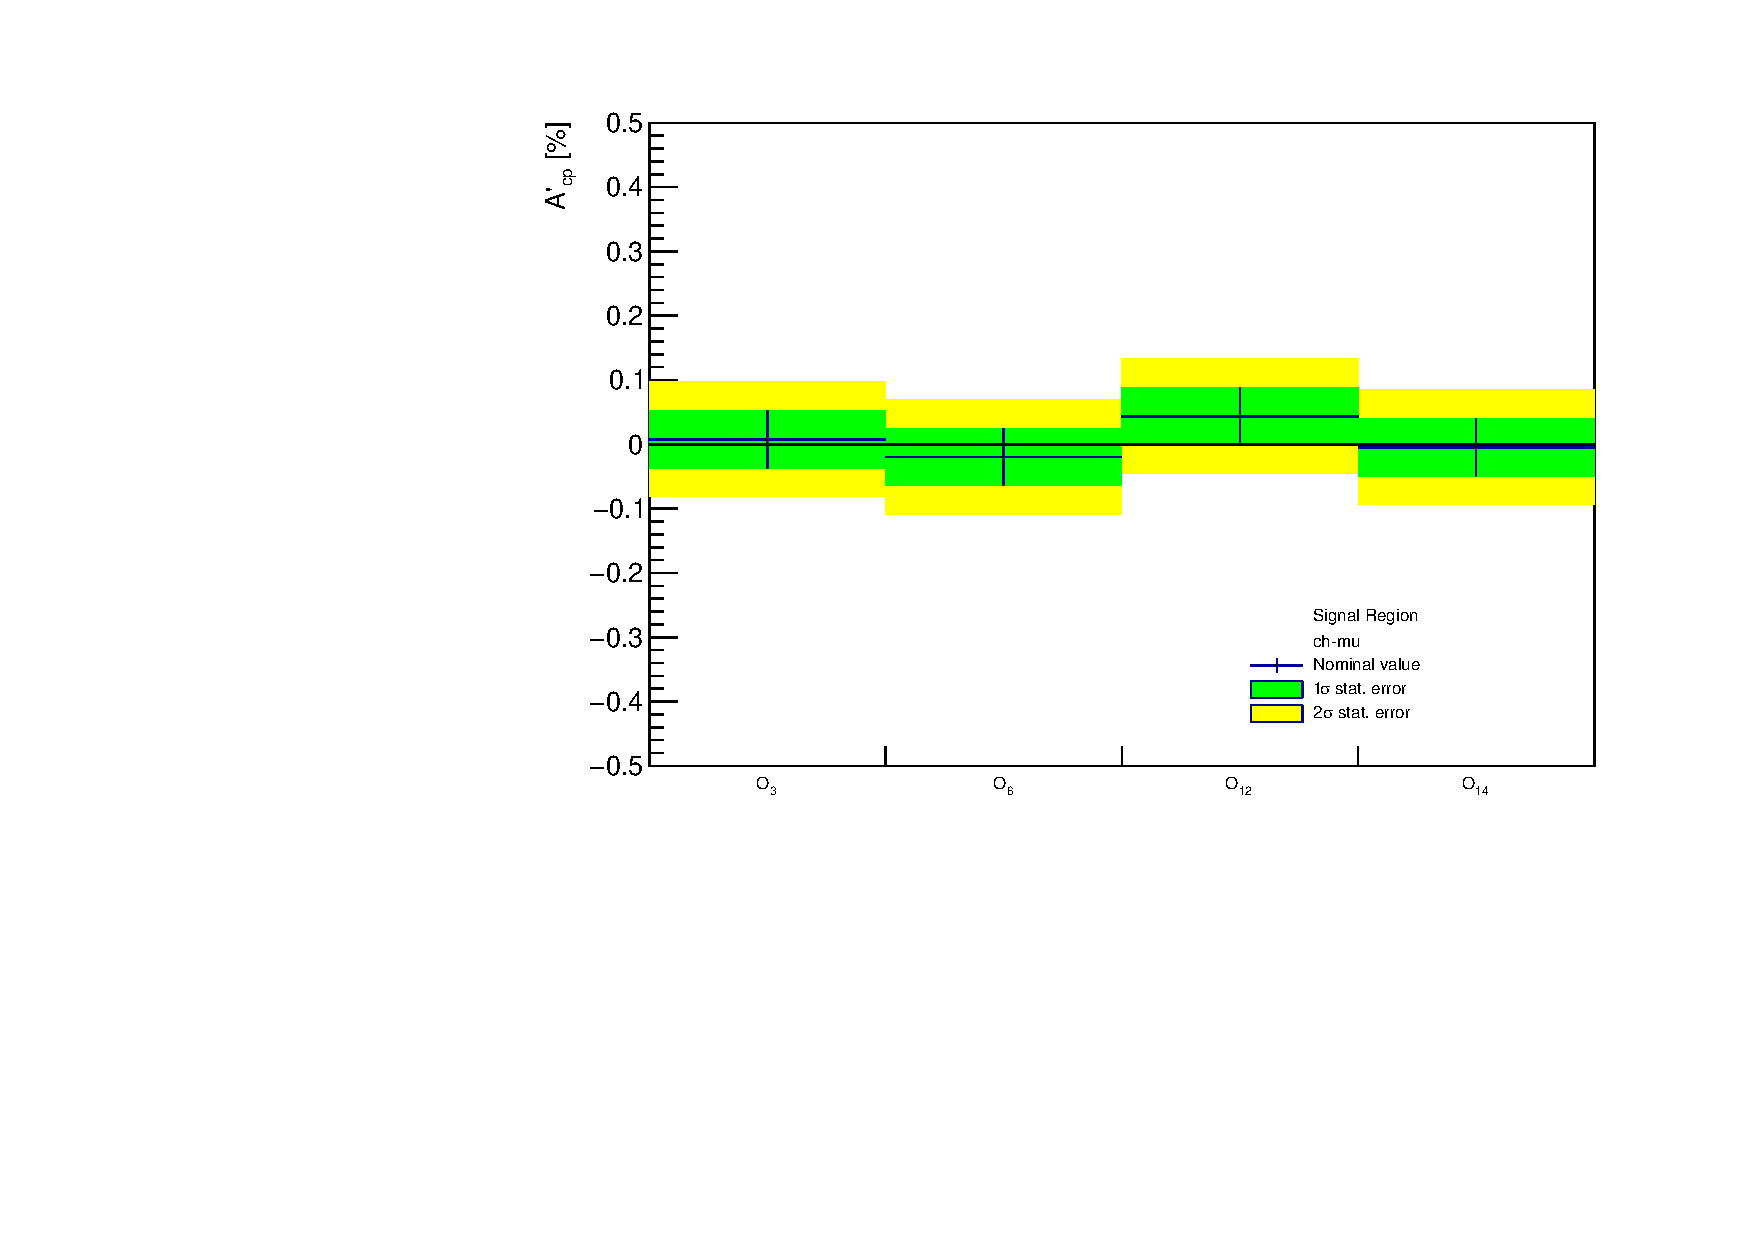
\includegraphics[width=0.45\textwidth]{Figures/Observables/TP_doublecheck/Acp_TP_semilep_genAcp_NoSel_10_7-semi_SM_i5_0j_mu.pdf}}
			    \subfigure[SM, Electron channel]{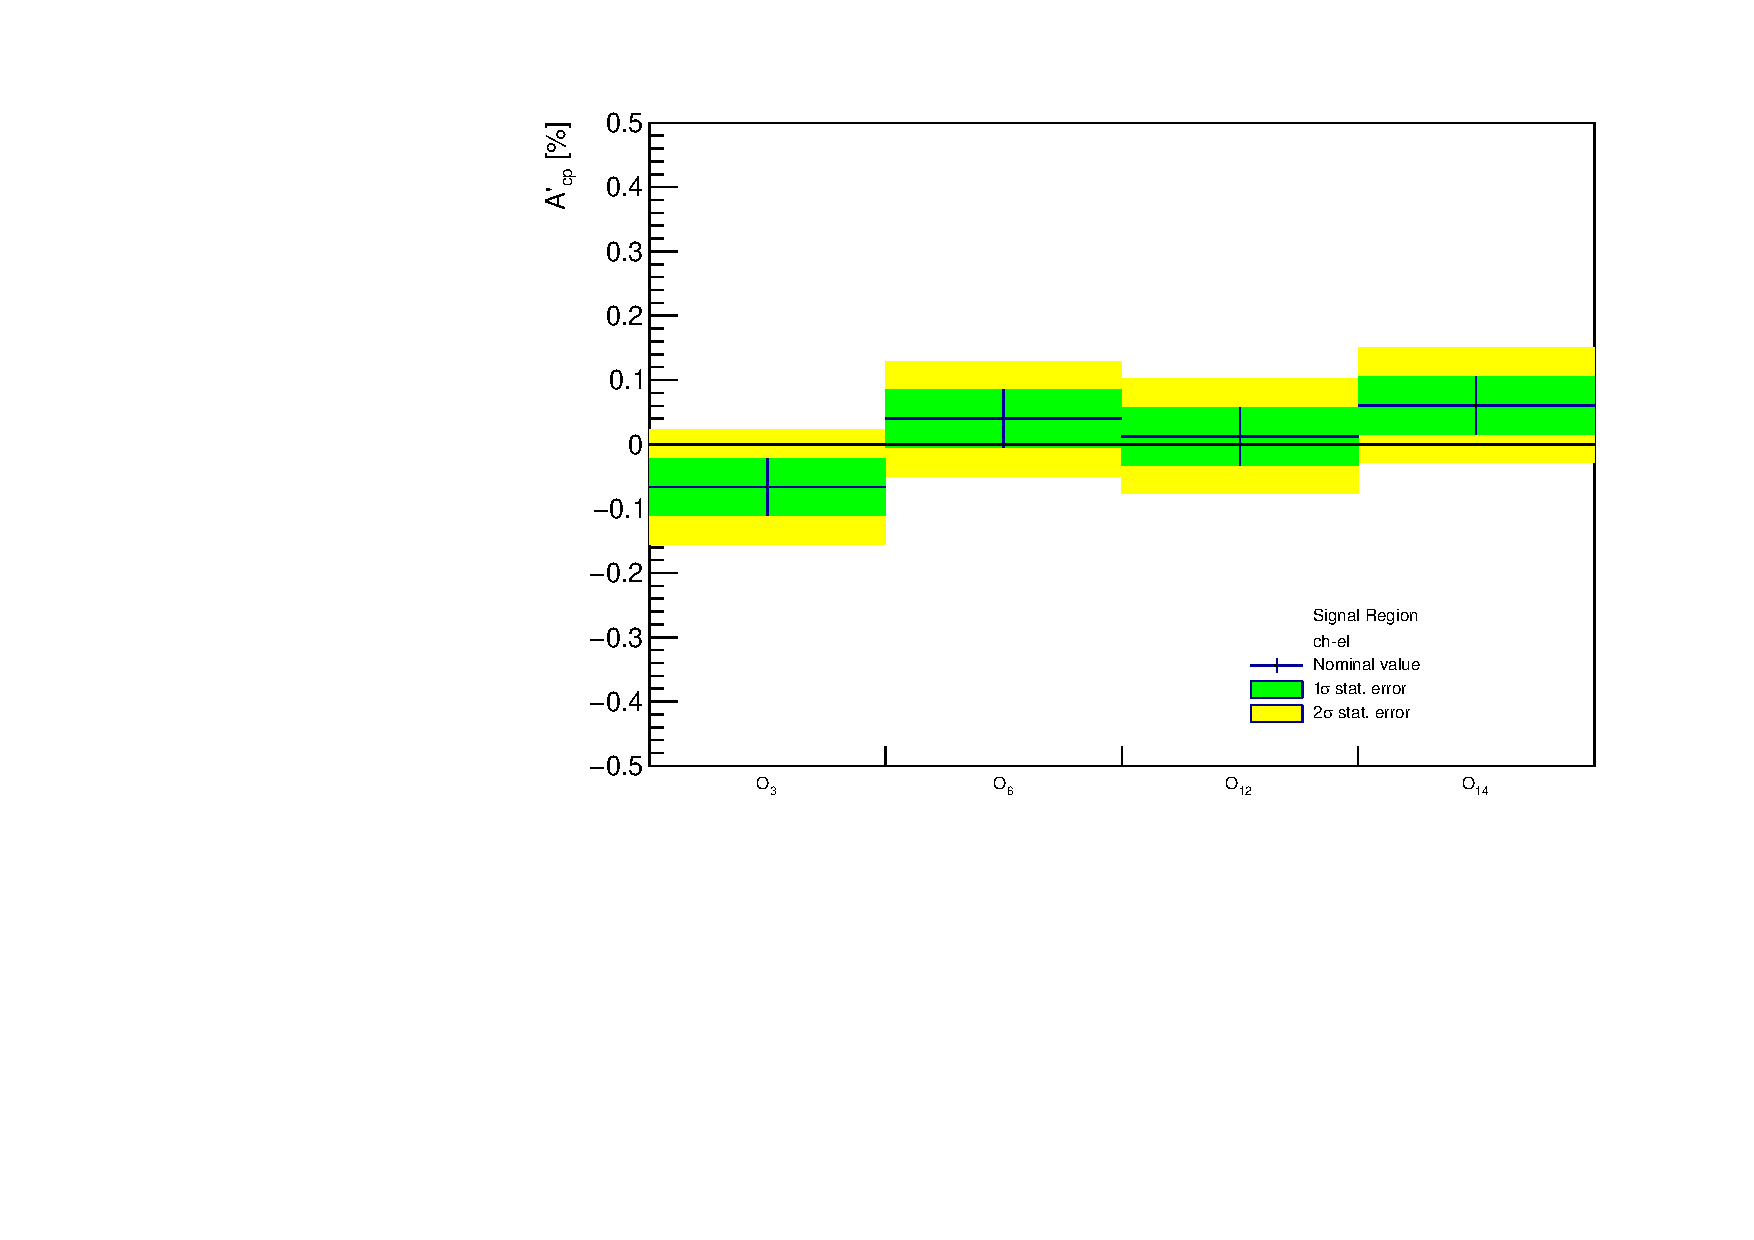
\includegraphics[width=0.45\textwidth]{Figures/Observables/TP_doublecheck/Acp_TP_semilep_genAcp_NoSel_10_7-semi_SM_i5_0j_el.pdf}}\\
			\end{figure}
			\FloatBarrier
			\begin{figure}[H]
			\centering
			    \subfigure[CEDM, Muon channel]{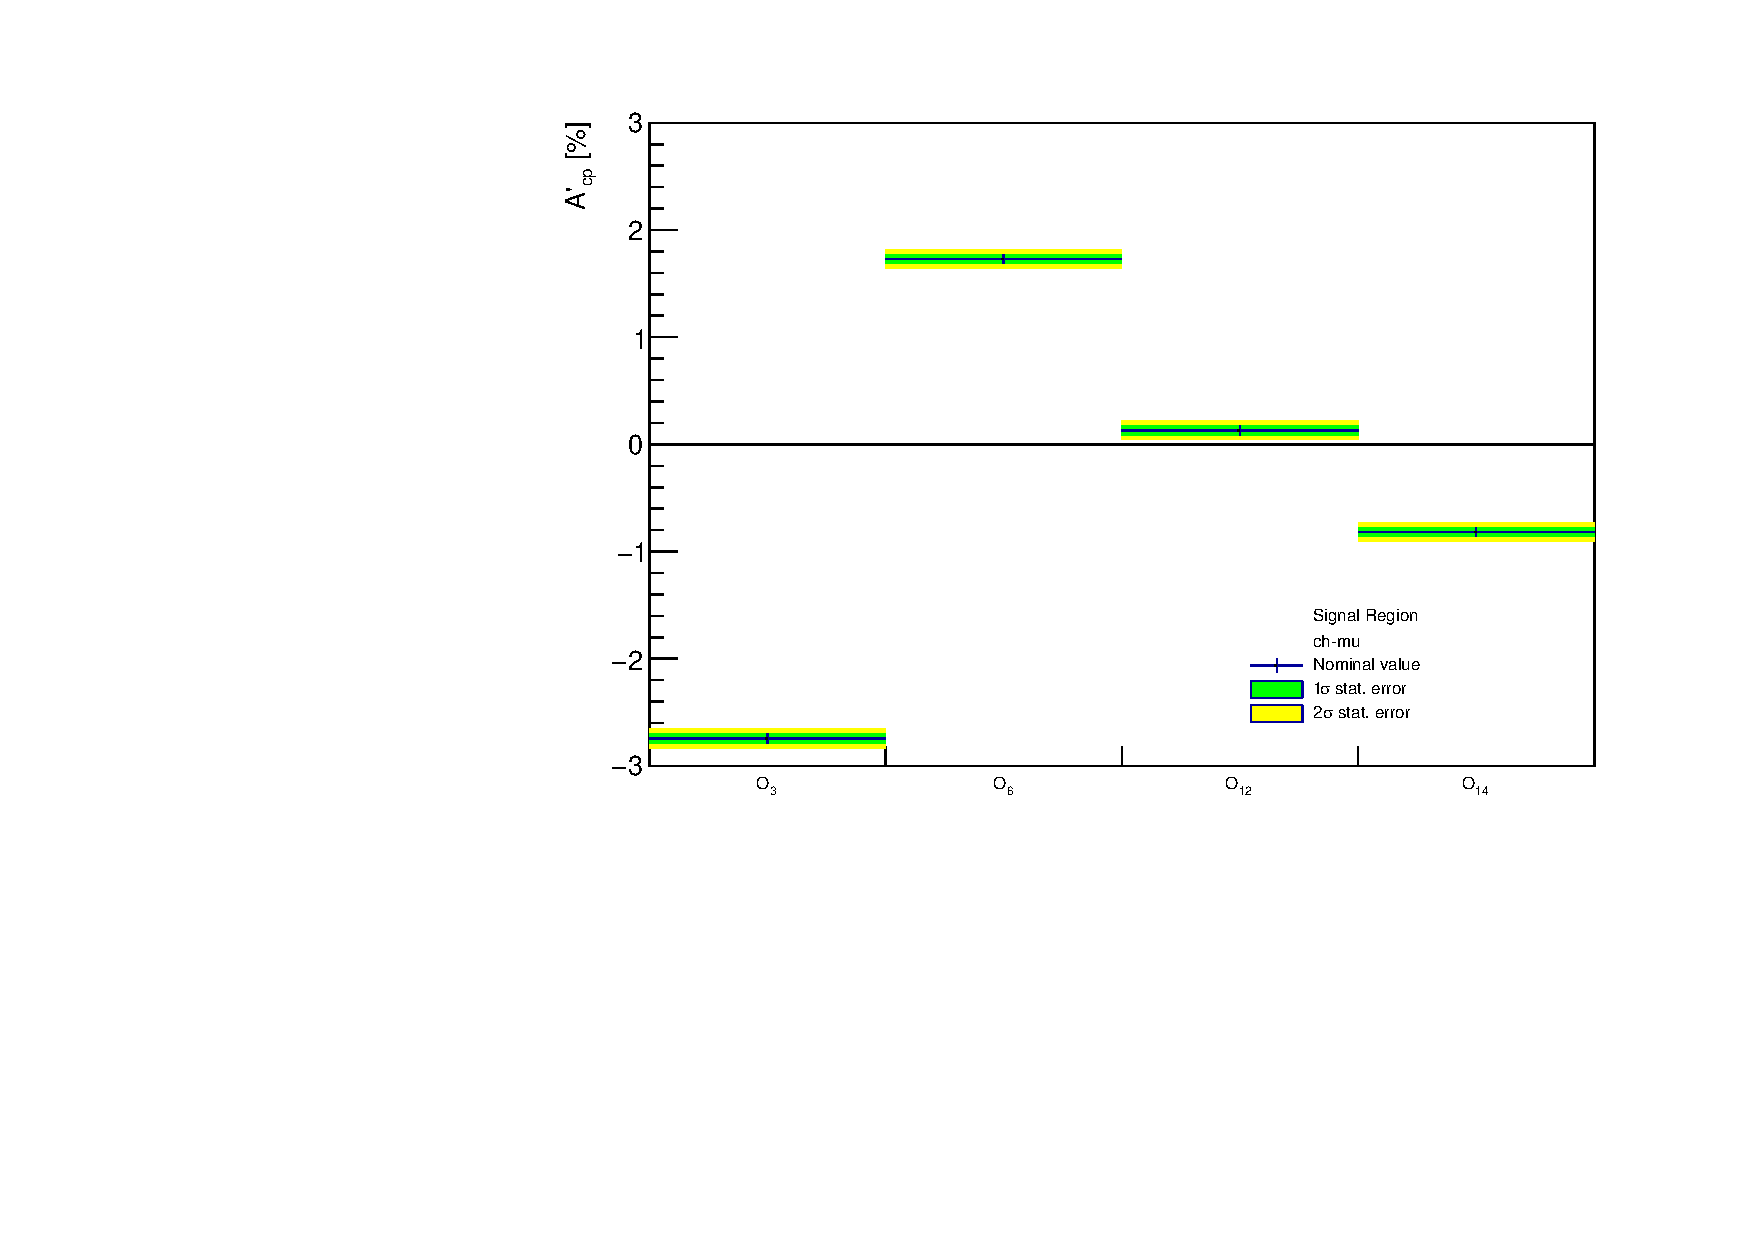
\includegraphics[width=0.45\textwidth]{Figures/Observables/TP_doublecheck/Acp_TP_semilep_genAcp_NoSel_10_7-semi_CEDM5_0j_mu.pdf}}
			    \subfigure[CEDM, Electron channel]{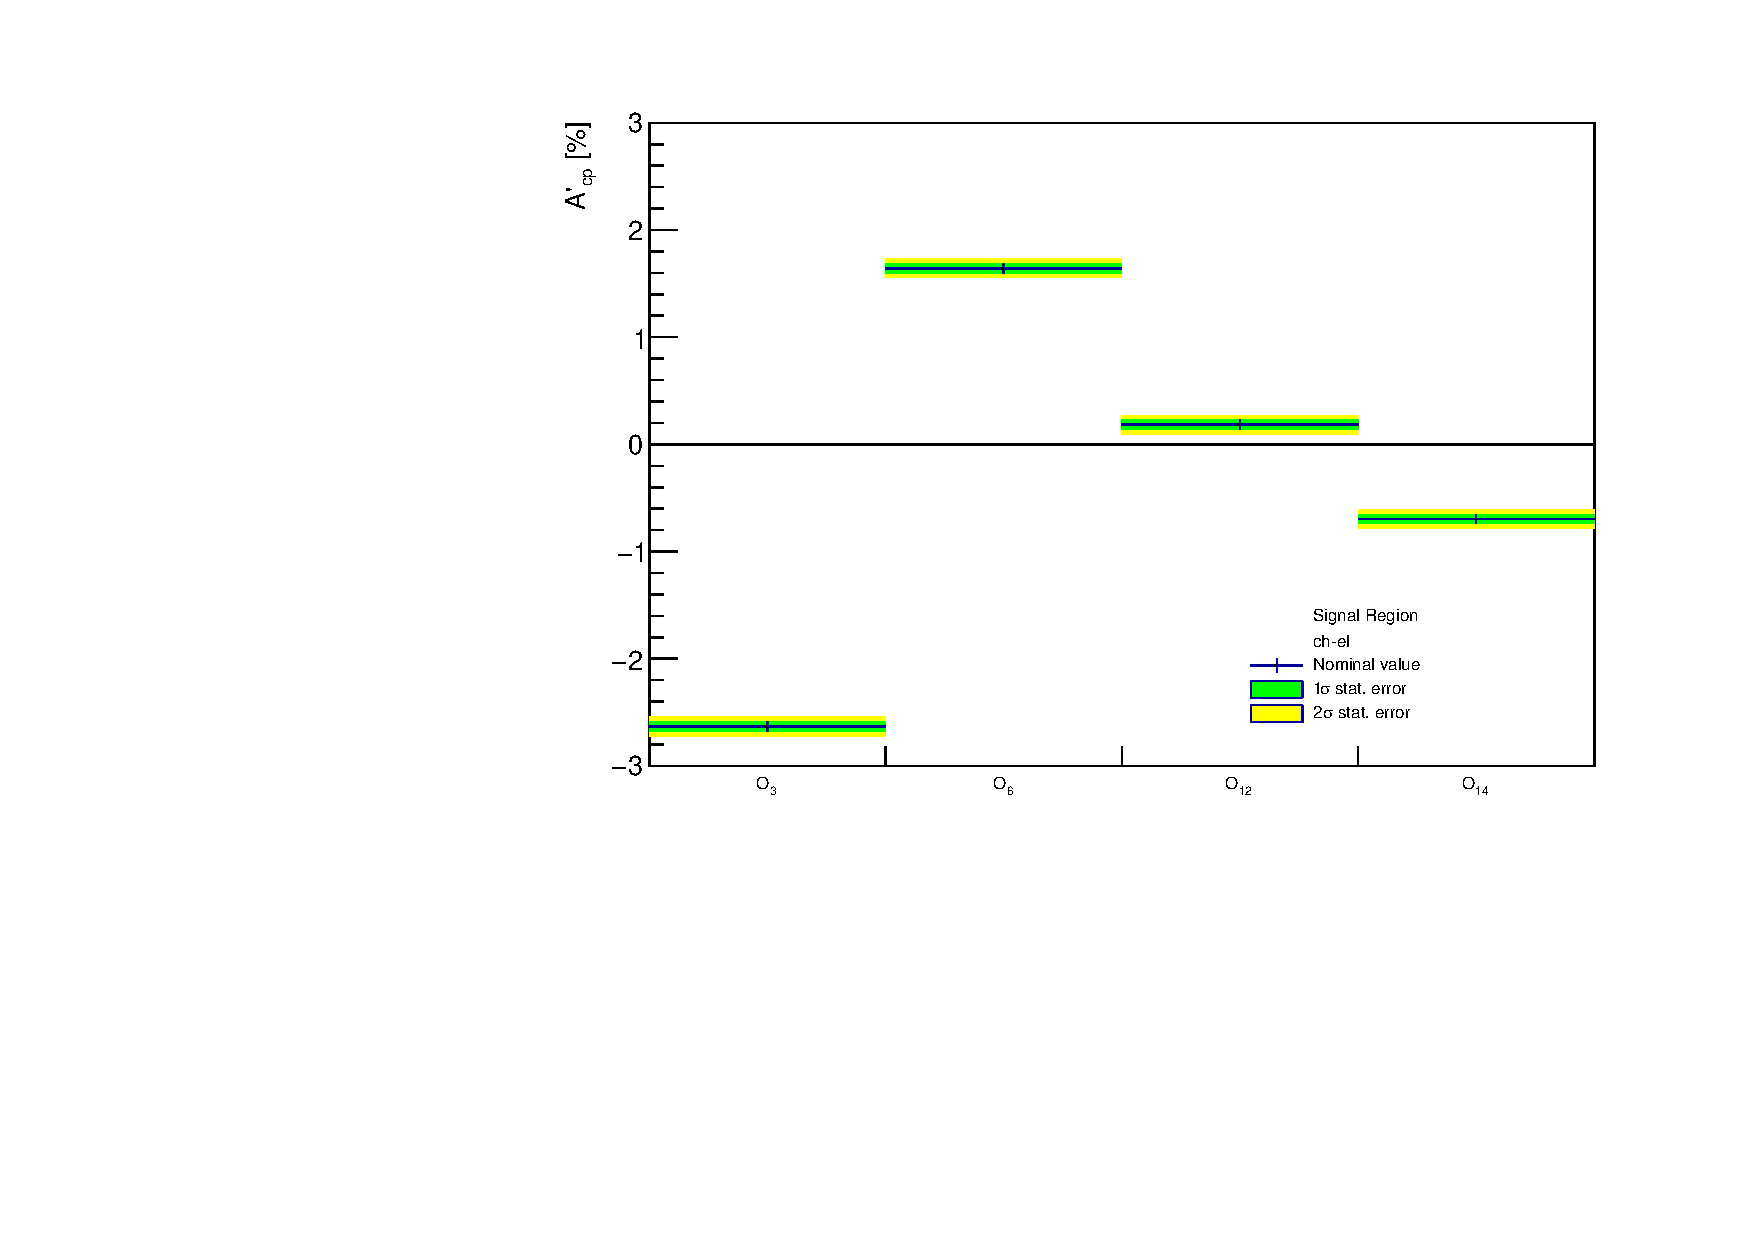
\includegraphics[width=0.45\textwidth]{Figures/Observables/TP_doublecheck/Acp_TP_semilep_genAcp_NoSel_10_7-semi_CEDM5_0j_el.pdf}}\\
			\end{figure}
			\FloatBarrier
			\begin{figure}[H]
			\centering
			    \subfigure[2HDM, Muon channel]{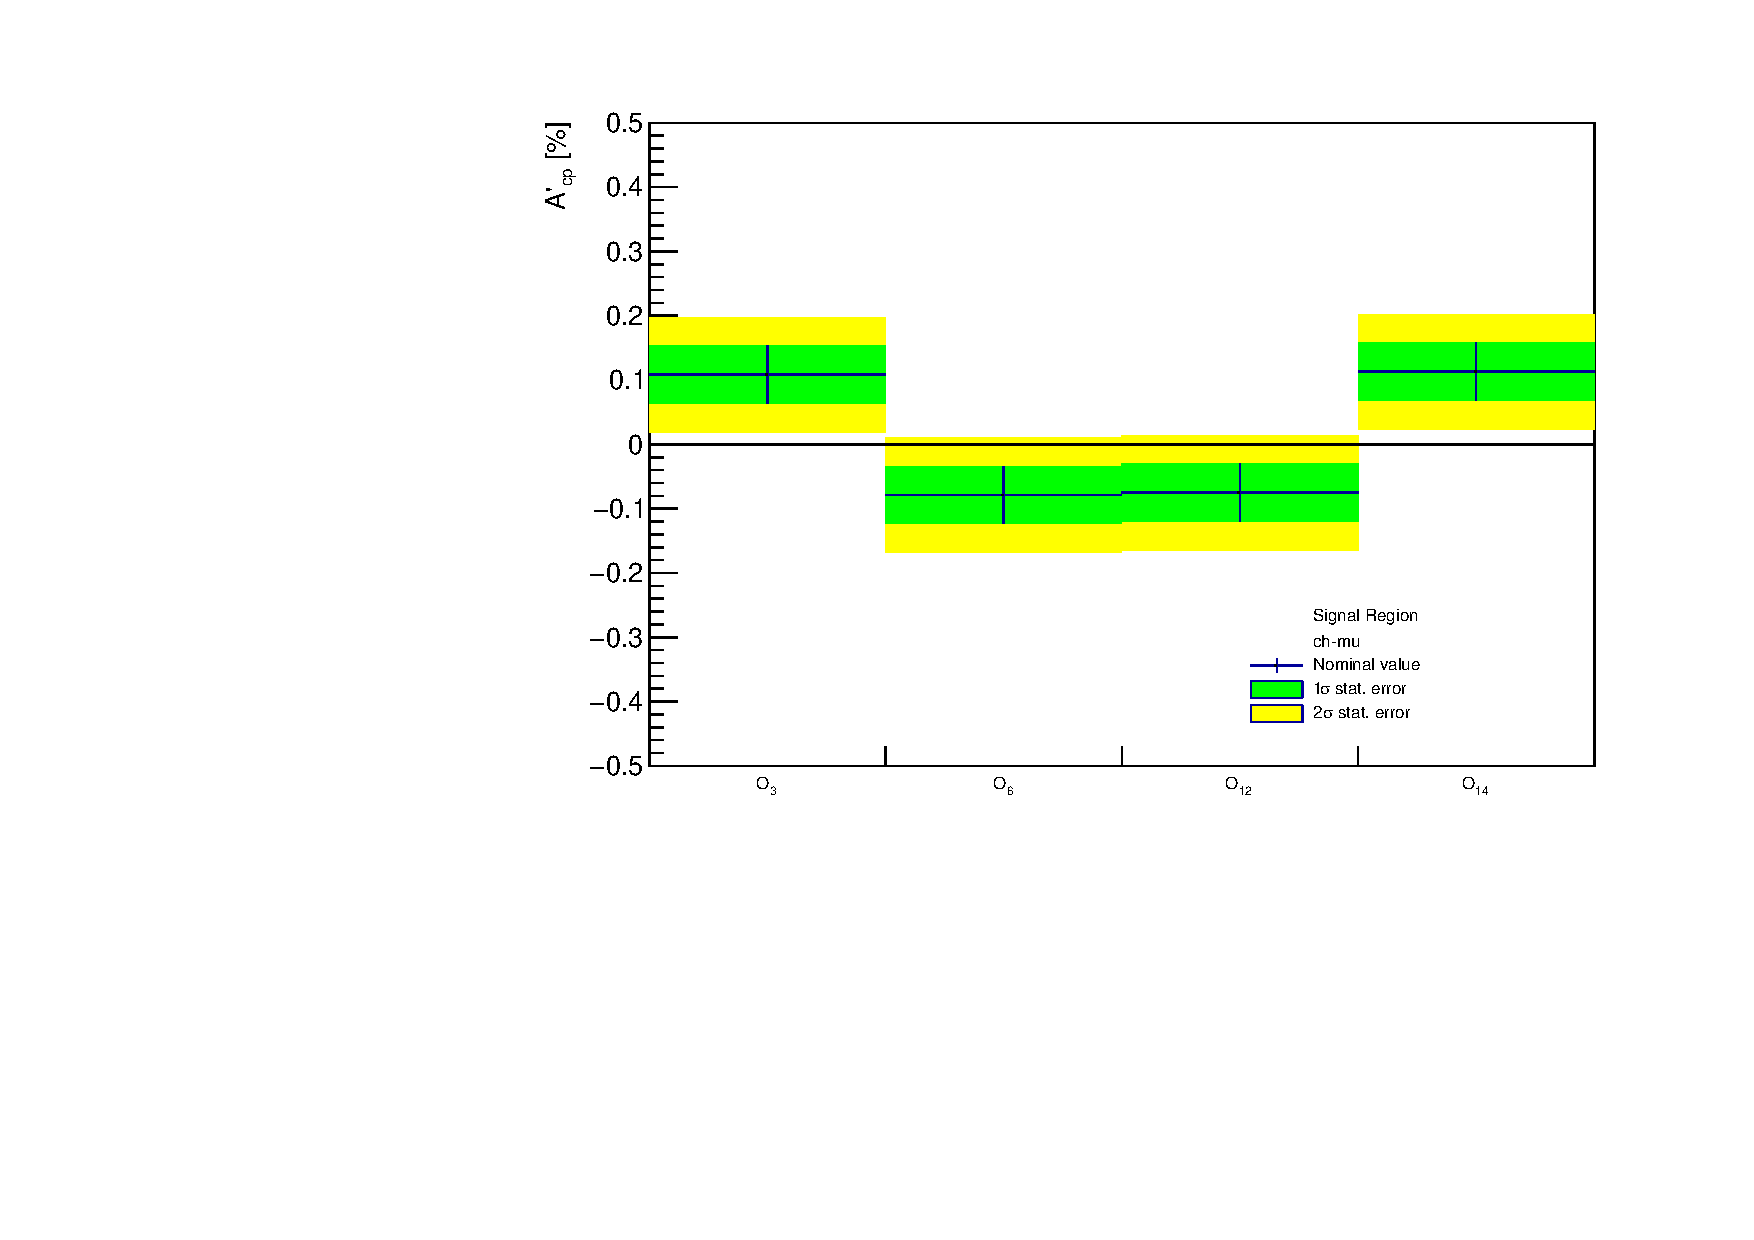
\includegraphics[width=0.45\textwidth]{Figures/Observables/TP_doublecheck/Acp_TP_semilep_genAcp_NoSel_10_7-semi_2HDM_NLO_m1_0j_mu.pdf}}
			    \subfigure[2HDM, Electron channel]{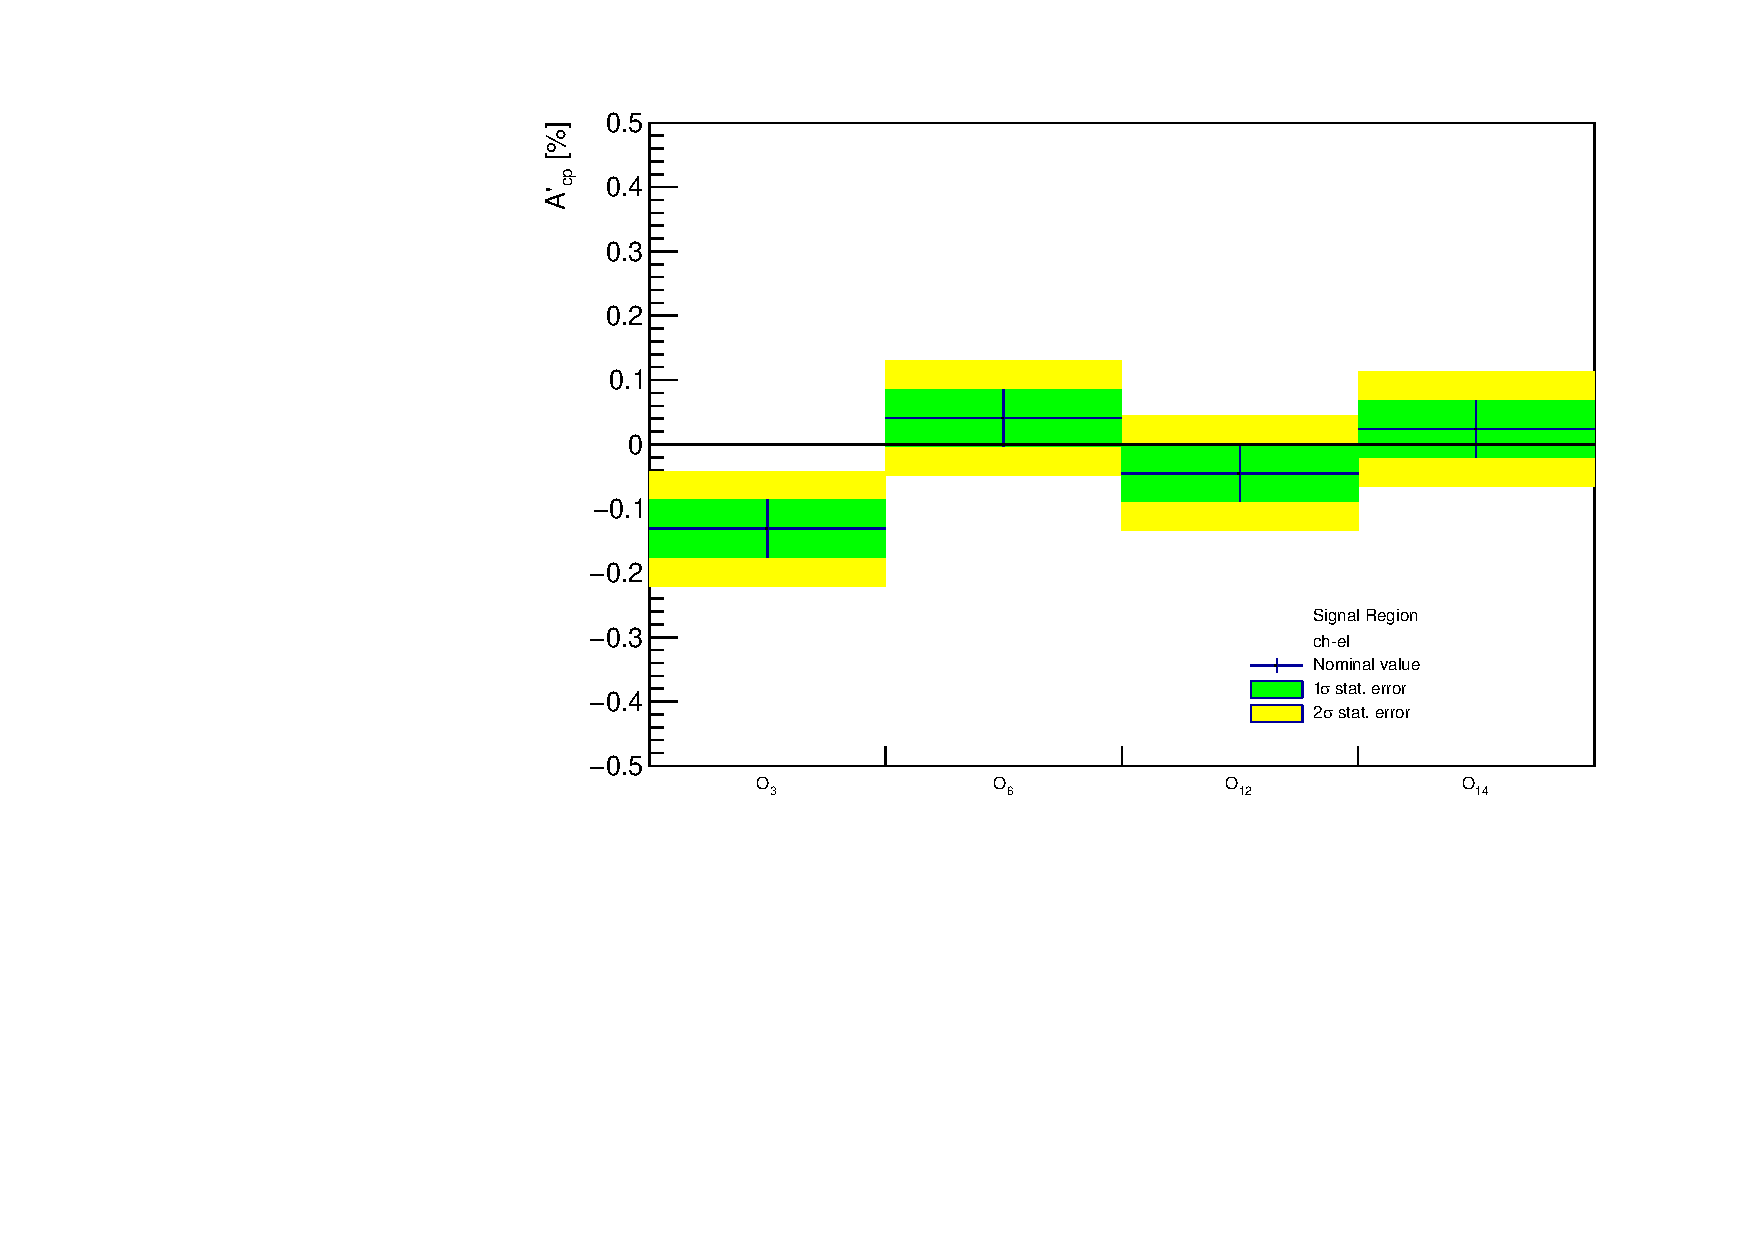
\includegraphics[width=0.45\textwidth]{Figures/Observables/TP_doublecheck/Acp_TP_semilep_genAcp_NoSel_10_7-semi_2HDM_NLO_m1_0j_el.pdf}}\\
			\caption{Measurement of three model's(SM, CEDM with $d_t^g=5$, 2HDM with default parameters setting) simulation sample with four triple product observables}
			\label{Obs:fig:TP_3model}
			\end{figure}
			\FloatBarrier

			Compared to the standard model's results -- the asymmetry values are supposely drop into 2 standard deviation range, the CEDM model shows great sensitivity to the triple product observables, and the 2HDM model with default parameter setting shows a little probability to be detect.

			Because of the extensive usage of triple-product-type observables, which is roughly equal to T-odd observales, to measure the asymmetry in $t\bar{t}$, we put emphasis on T-even observable here. 

			% Peskin
			The first one is from \cite{PhysRevLett.69.410}. It is also researched with Higgs sector, exchange of Higgs boson $\phi$ creates CP-violating final-state interactions in $t\bar{t}$ by gluons or quarks. It is stated that the helicity conservation insists that gluons mainly produce left-handed top quarks($t_L$) accompanying with right-handed anti-top quarks($\bar{t}_R$) and vice versa($t_R$ with $\bar{t}_L$). Yet, there is also production of $t_L \bar{t}_L$ and $t_R \bar{t}_R$ going into each other under CP. The diffrence of the two production rate would be the signal of CP violation. Then it leads to a charge asymmetry in the energy distribution of decaying W from top quarks otr their decay leptons. The $t\bar{t}$ asymmetry mentioned in this paper is shown:

			\begin{equation}
			\Delta N_{LR} = [N(t_L \bar{t}_L)-N(t_R \bar{t}_R)]/N(all \; t\bar{t})
			\label{eq:SP_001}
			\end{equation}

			The CP-violating polarization asymmetry would be translated in the energy spectra of charged leptons from top decay. Below is the decay distribution of the charged lepton.(Eq.\ref{eq:SP_002})
			
			\begin{equation}
			\frac{d^2 \Gamma}{d E_l d \cos{\psi}} = \frac{d \Gamma}{d E_l} \frac{ 1 + \cos{\psi}}{2} 
			\label{eq:SP_002}
			\end{equation}

			where the $\psi$ is the angle between the lepton's momentum and the top spin, the $d\Gamma/dE_l$ is the unpolarized energy distribution. When the top quark is boosted, Eq.\ref{eq:SP_002} give a correlation between top helicity and lepton energy. Then the lepton energy is exactly an appropriate $t$ spin analyzer. The adaptation from energy to tranverse energy is to avoid the effects of longitudinual boost of the parton-parton collision. There are shown the asymmetry would occur on the spectrum of transverse energy difference between positive lepton and negative lepton by $\Delta N$:

			\begin{equation}
			\Delta N(E_T) = \frac{d\sigma/dE_{T,l^{+}} - d\sigma/dE_{T,l^{-}}}{d\sigma/dE_{T,l^{+}} + d\sigma/dE_{T,l^{-}}}
			\label{eq:SP_003}
			\end{equation}

			The CP violation and comparising non-CP-violating cases would be shown in Fig.\ref{Obs:fig:SP_ex}

			\begin{figure}[H]
			\centering
			    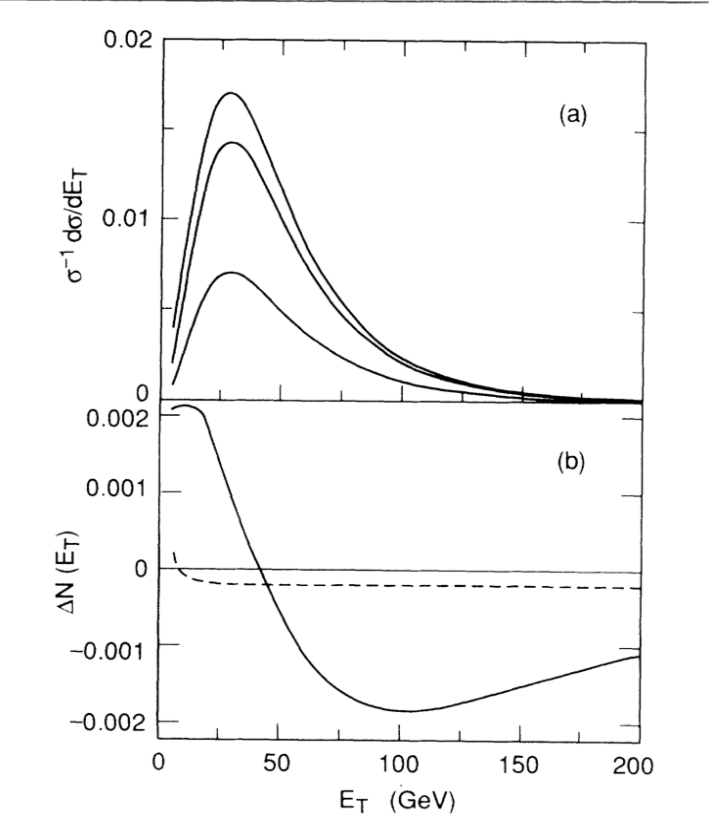
\includegraphics[width=0.45\textwidth]{Figures/Observables/SchmidPeskin.png}
			\caption{Upper diagram shows the transverse energy distribution of positive/negative leptons of generated sample. The lower plots show the $\Delta N$ under the $E_T$ spectrum. The dashed line result is due to non-CP-violating effects and the solid line is due to CP violation.}
			\label{Obs:fig:SP_ex}
			\end{figure}
			\FloatBarrier

			With the rough criteria, there are just some test with this lepton asymmetry observable by Madgraph generated SM, CEDM($d_t^g = 5$), 2HDM(default setting) $t\bar{t}$ samples with no selection and $10^7$ events. I test both on $t\bar{t}$ dilepton decay and semi-leptonic decay. It is just that collecting both leptons from dilepton decay and that collecting one lepton in each semileptonic decay event. 

			\begin{figure}[H]
			\centering
			    \subfigure[dilepton decay $t\bar{t}$, SM]{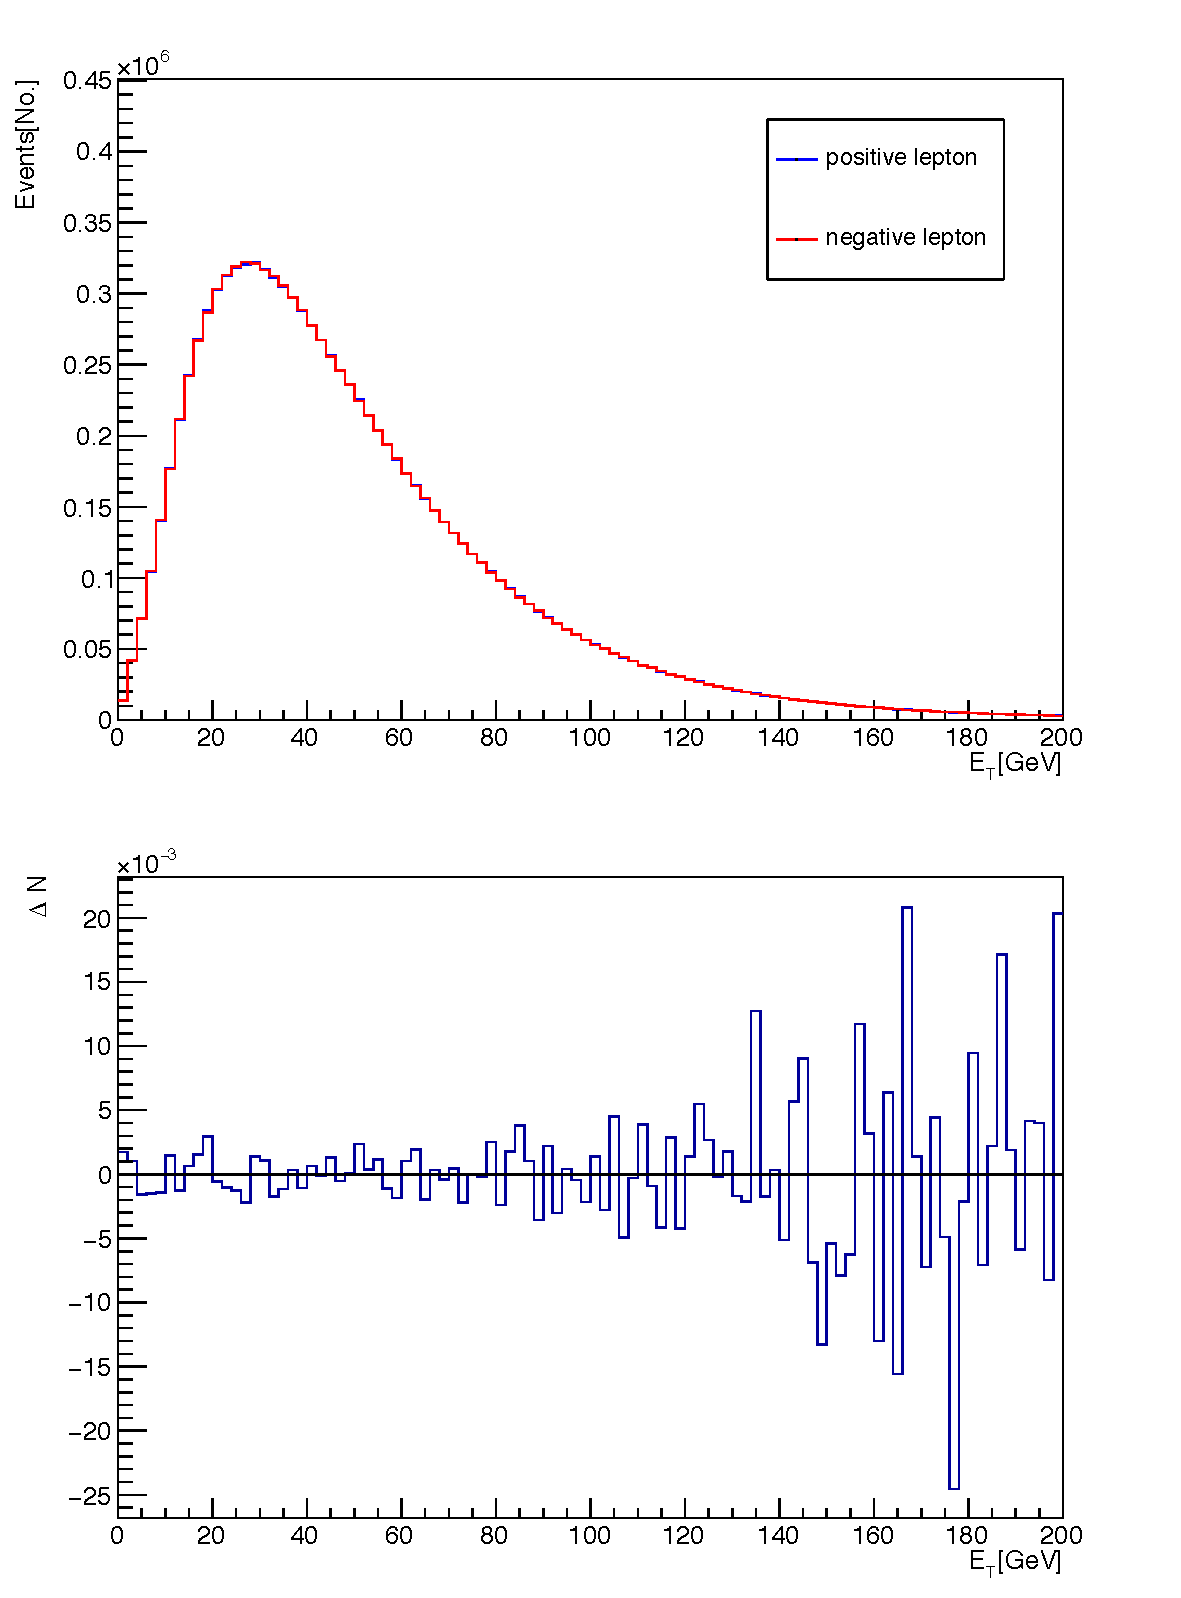
\includegraphics[width=0.32\textwidth]{Figures/Observables/lepEtAsym_10_7-dilep_SM_0j_NoSel_comb.pdf}}
			    \subfigure[dilepton decay $t\bar{t}$, CEDM]{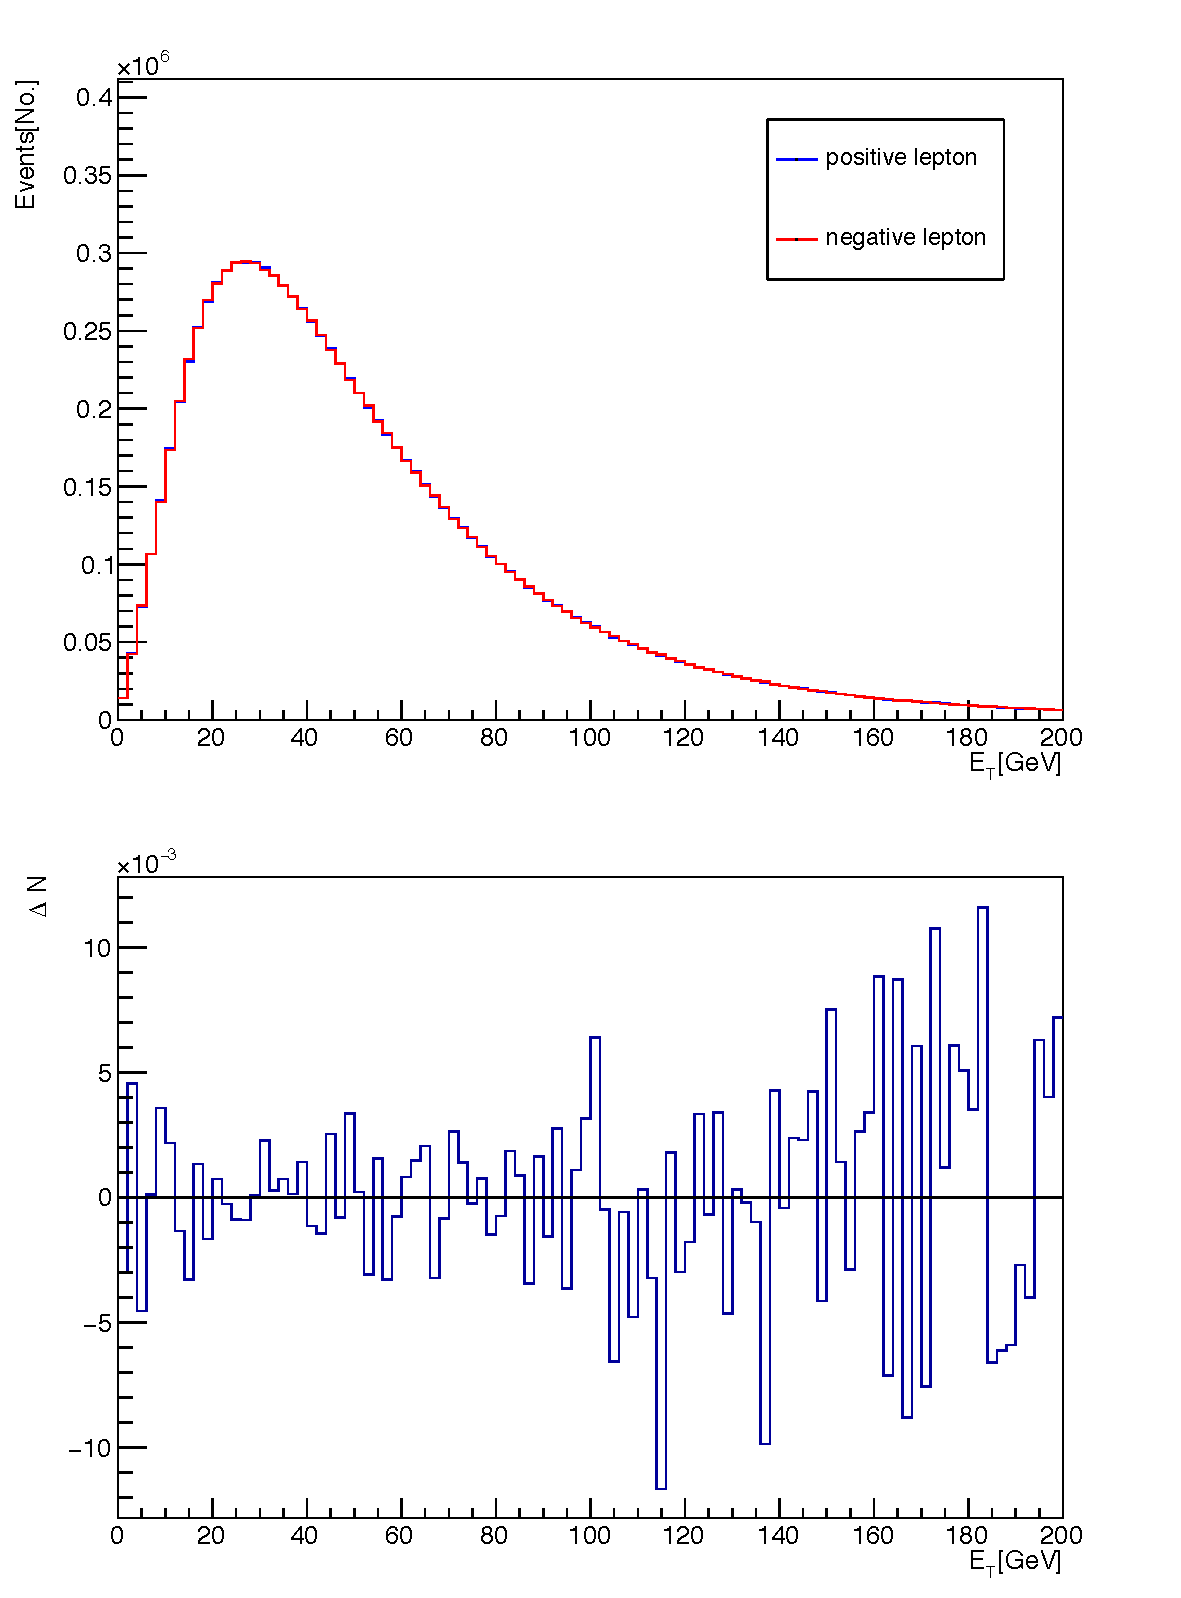
\includegraphics[width=0.32\textwidth]{Figures/Observables/lepEtAsym_10_7-dilep_CEDM5_0j_NoSel_comb.pdf}}
			    \subfigure[dilepton decay $t\bar{t}$, 2HDM]{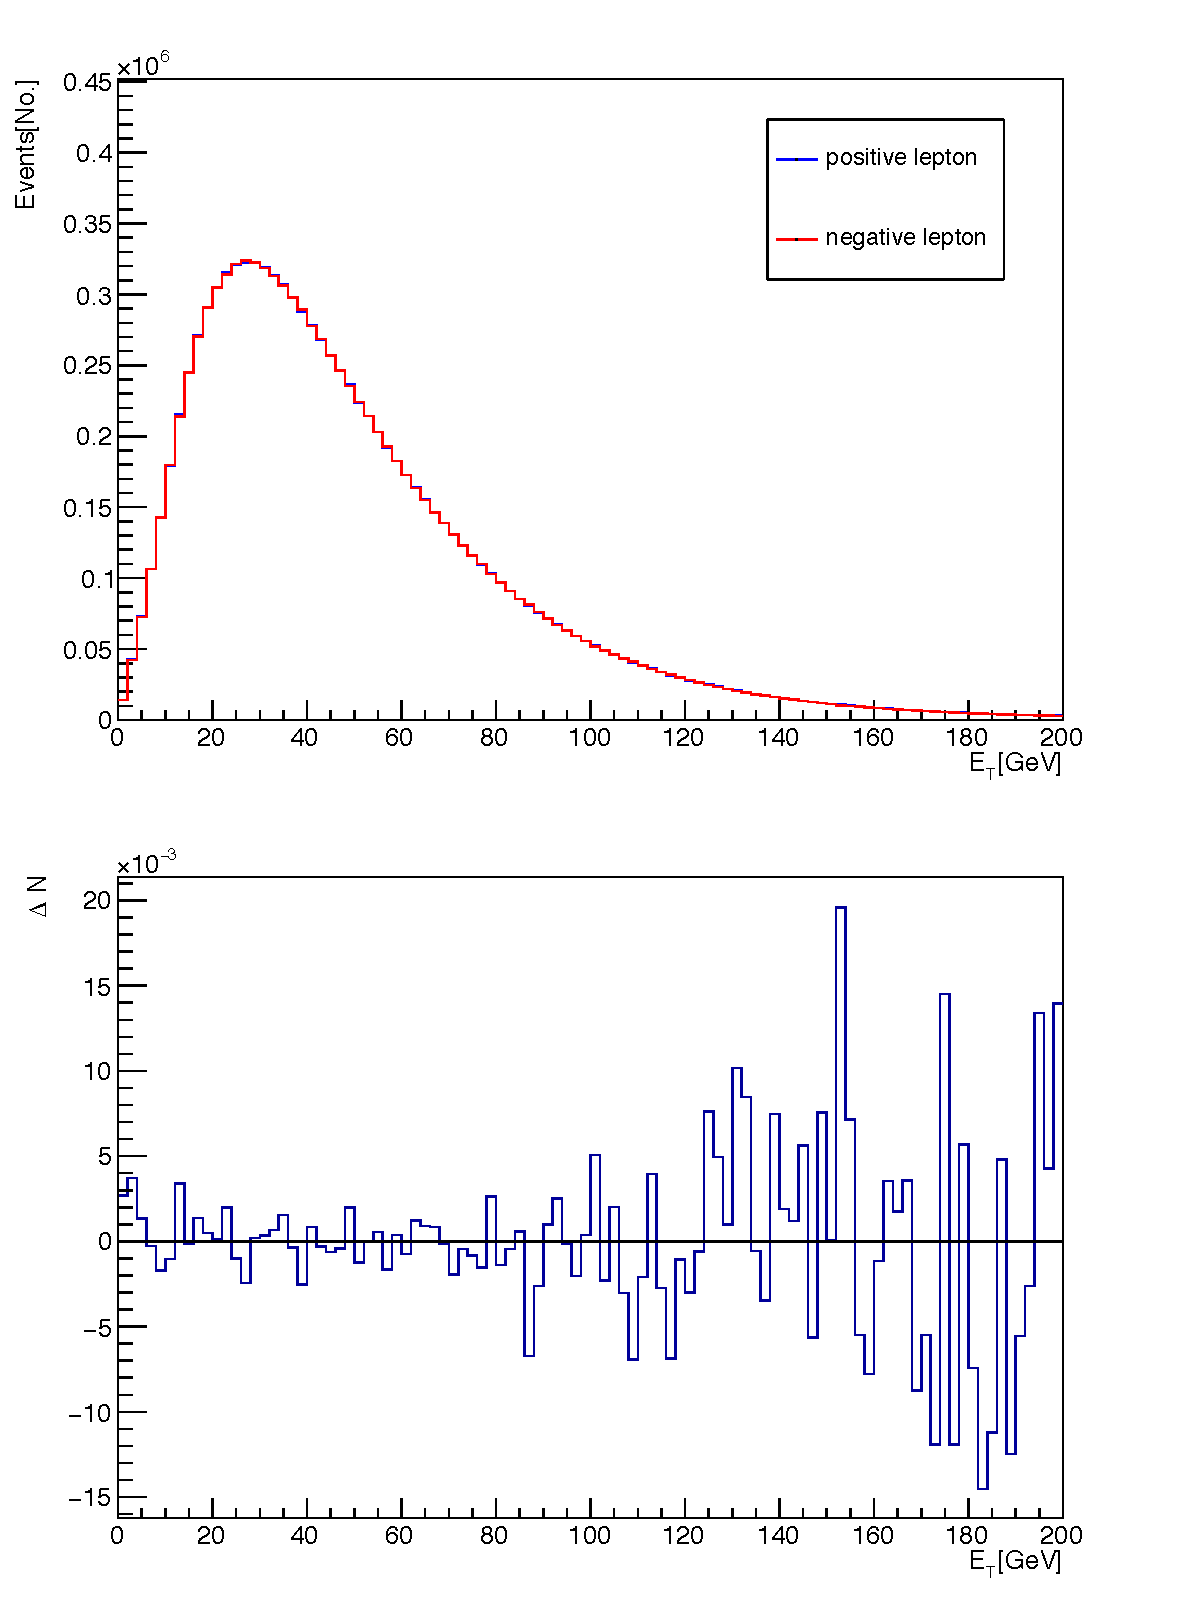
\includegraphics[width=0.32\textwidth]{Figures/Observables/lepEtAsym_10_7-dilep_2HDM_NLO_m1_0j_NoSel_comb.pdf}}\\
			\end{figure}
			\FloatBarrier
			\begin{figure}[H]
			\centering
				\subfigure[semi-leptonic decay $t\bar{t}$, SM]{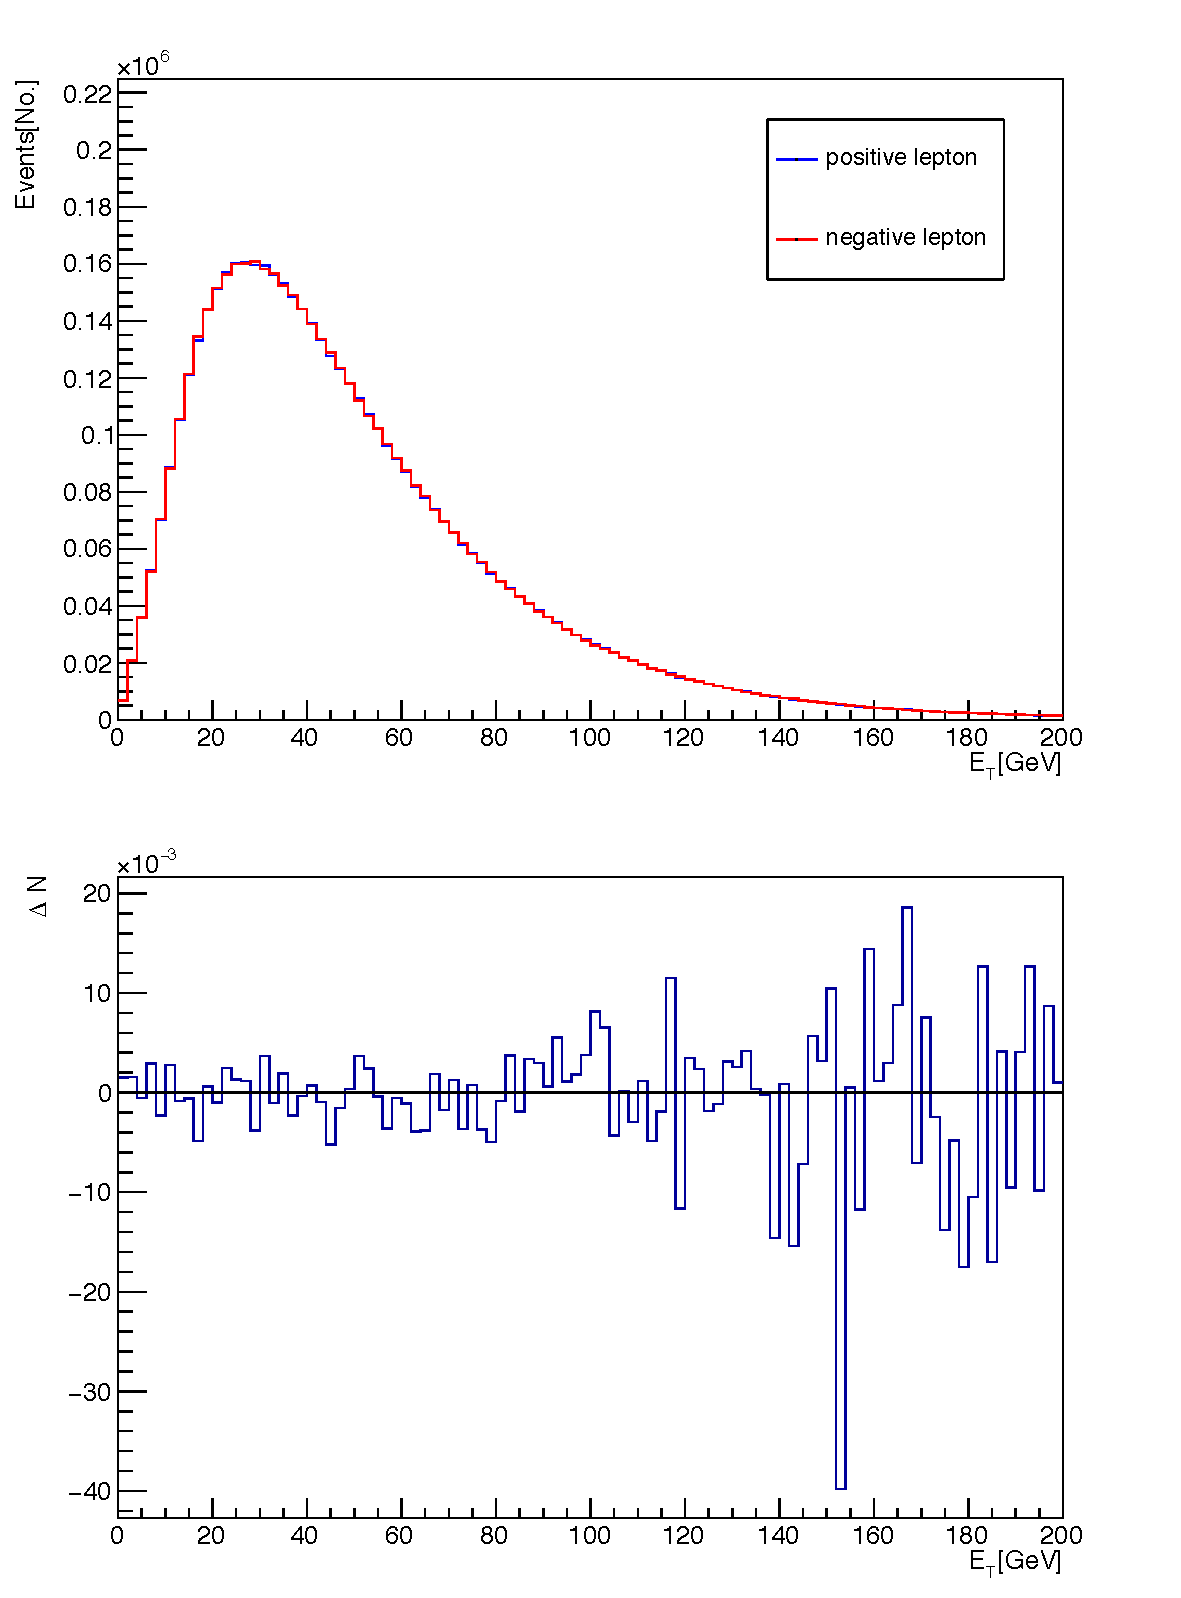
\includegraphics[width=0.32\textwidth]{Figures/Observables/lepEtAsym_10_7-semi_SM_0j_NoSel_comb.pdf}}
			    \subfigure[semi-leptonic decay $t\bar{t}$, CEDM]{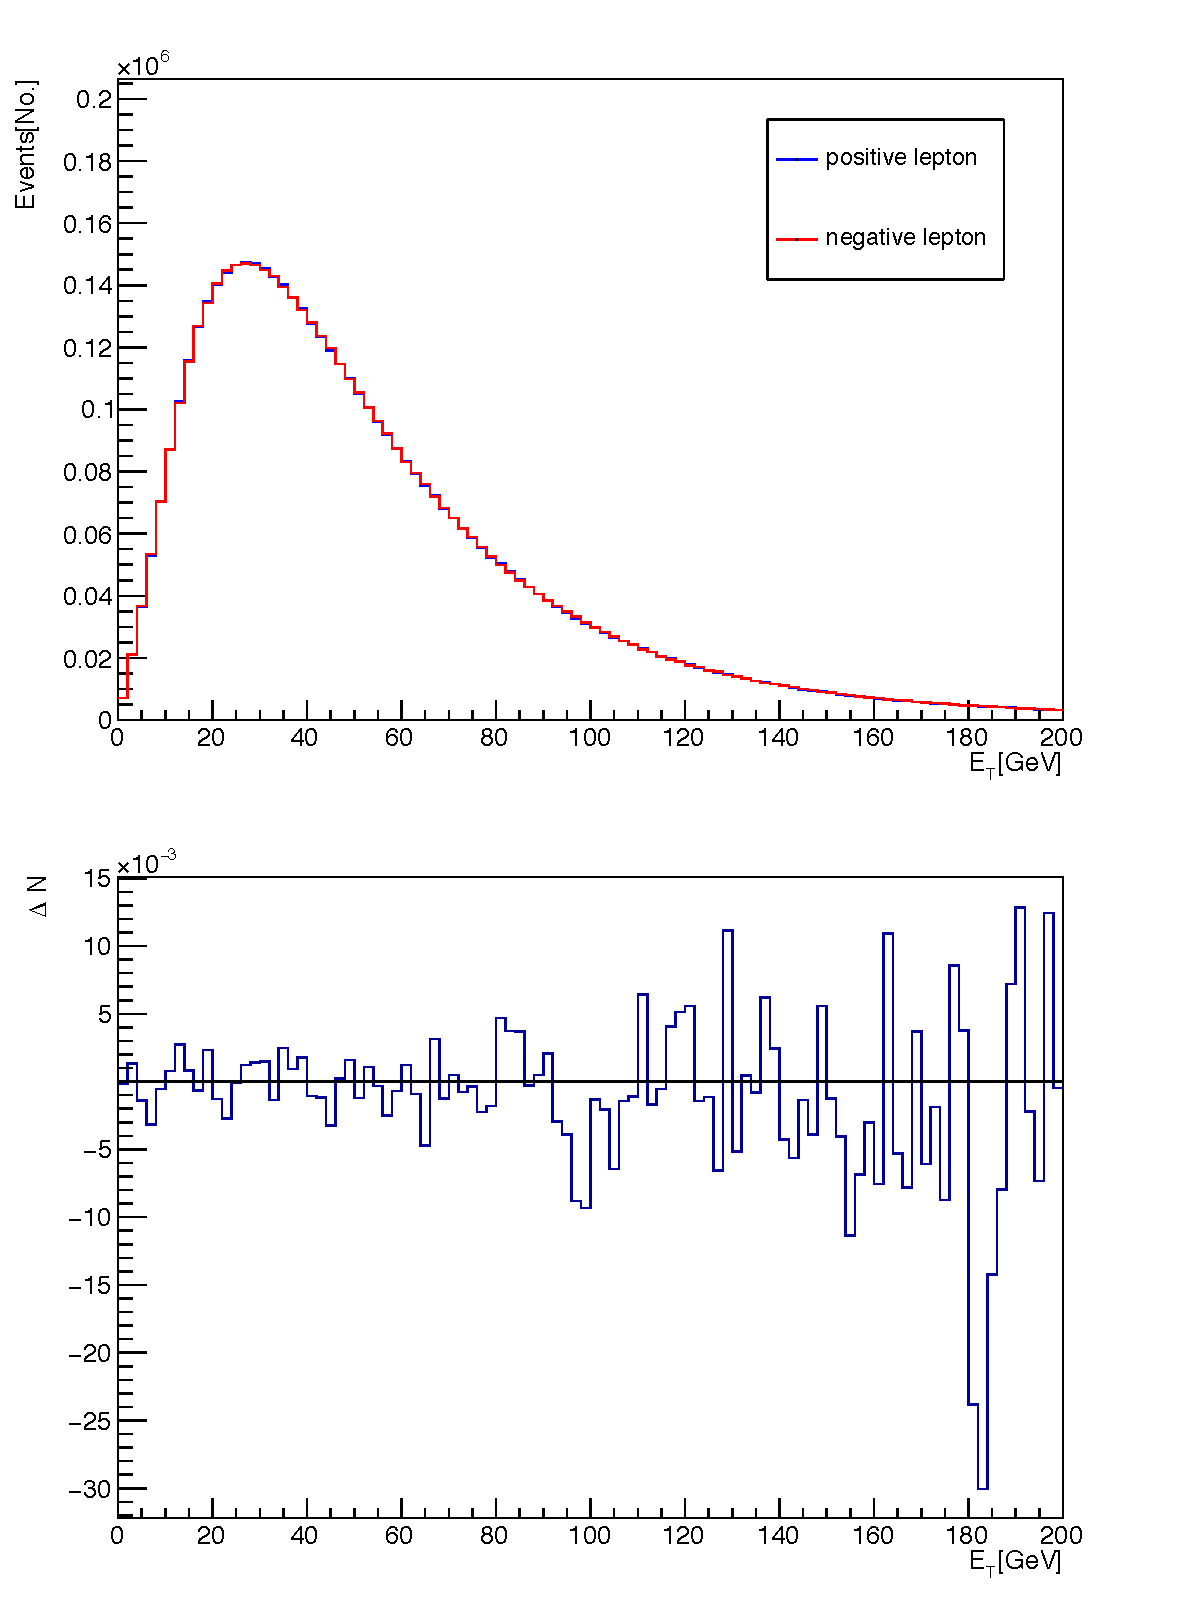
\includegraphics[width=0.32\textwidth]{Figures/Observables/lepEtAsym_10_7-semi_CEDM5_0j_NoSel_comb.pdf}}
			    \subfigure[semi-leptonic decay $t\bar{t}$, 2HDM]{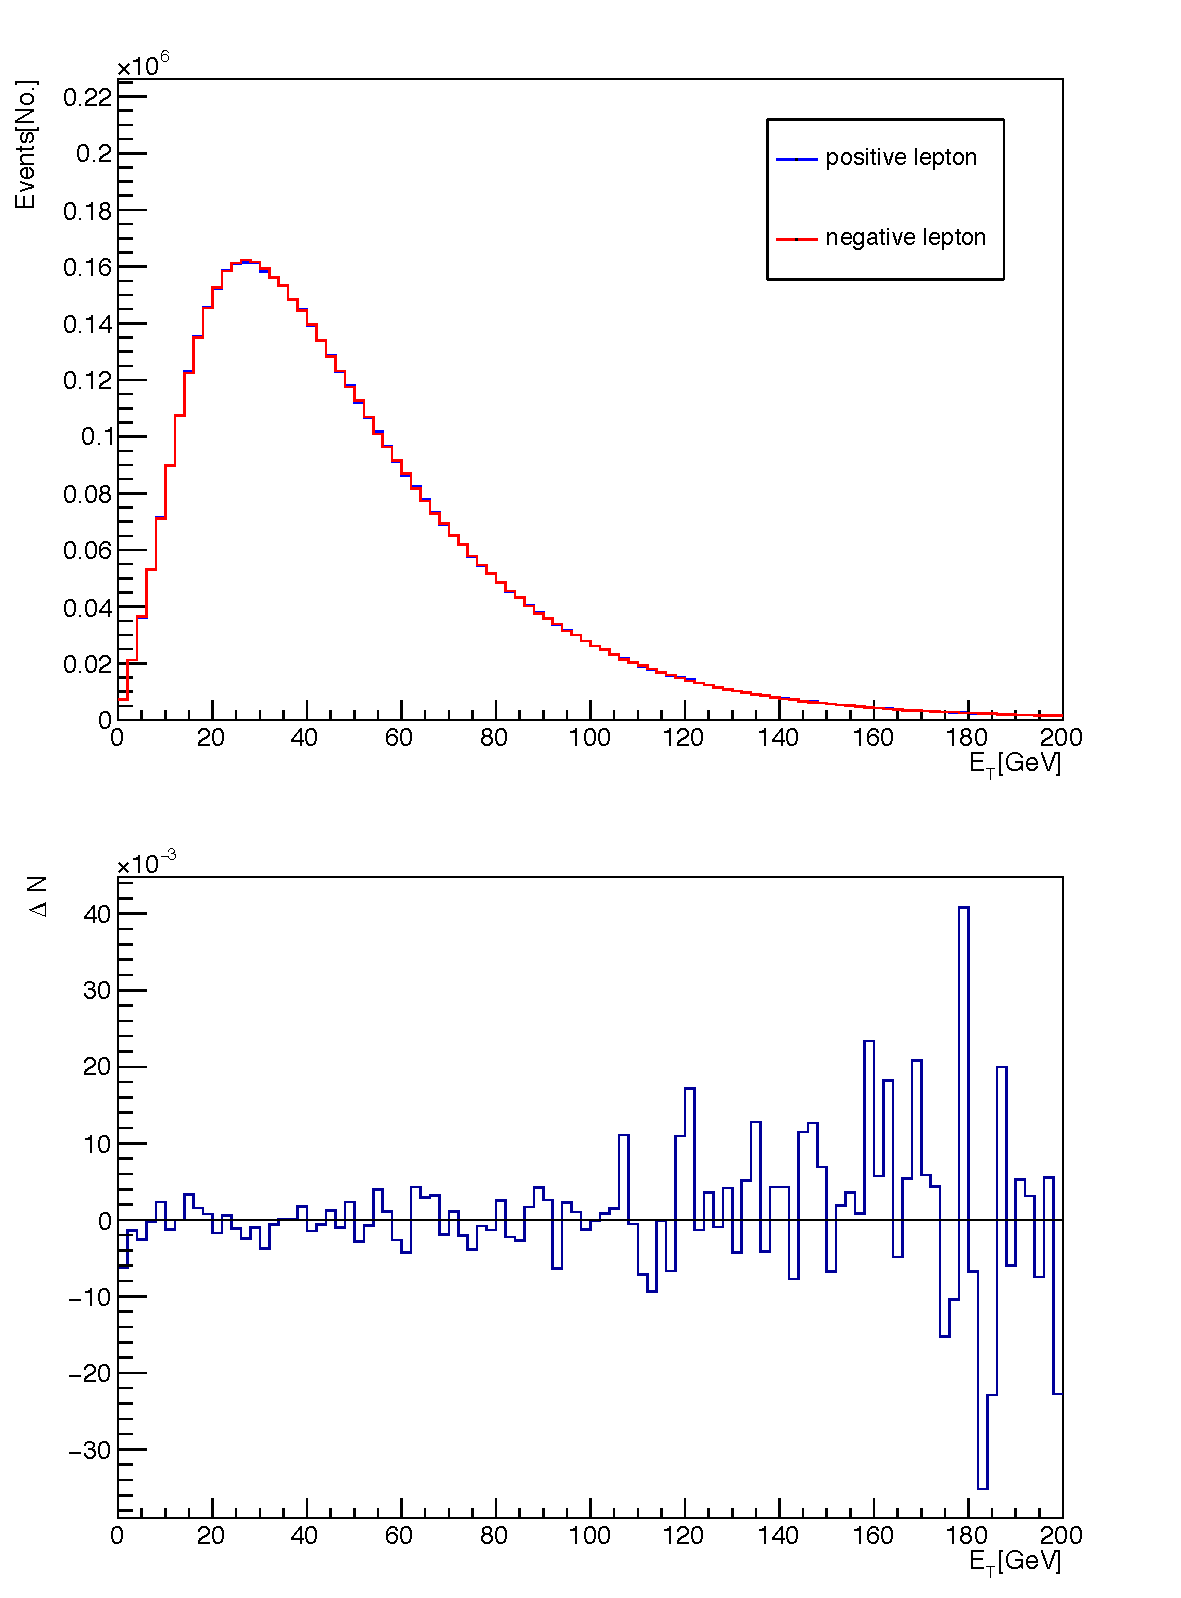
\includegraphics[width=0.32\textwidth]{Figures/Observables/lepEtAsym_10_7-semi_2HDM_NLO_m1_0j_NoSel_comb.pdf}}\\
			\caption{The positive and negative leptons' $E_T$ distribution and $\Delta N$ with dilepton and semileptonic decay simulated $t\bar{t}$, with 3 models(SM, CEDM, 2HDM)}
			\label{Obs:fig:}
			\end{figure}
			\FloatBarrier

			There are not obvious asymmetry and precise standard under the observable.

			% B&B 1993
			Second, in the paper\cite{Bernreuther:1993hq}, when discussing the 2HDM model, they state that using the expectation value of an observable $O$(Eq.\ref{eq:1993_001}) to identify the correlations at the parton level which trace the CP-odd parts of the $t\bar{t}$ production density matrices.
			
			\begin{equation}
			<O_i> = \frac{\int_{-1}^{1}dz\cdot tr(R^iO)}{4\int_{-1}^{1}dz\cdot A^i}\;\;,\;\;\;\;(i=g,q) 
			\label{eq:1993_001}
			\end{equation}

			Contributions to the observables have 2 types form and their linear combination:(Eq.\ref{eq:1993_002})

			\begin{equation}
			\begin{split} 
			\hat{\textbf{k}} \cdot (s_+ - s_-) f_e(z) \\
			\hat{\textbf{p}} \cdot (s_+ - s_-) f_0(z)
			\end{split}
			\label{eq:1993_002}
			\end{equation}

			where $s_+$, $s_-$ arre the spin operators of $t$ and $\bar{t}$. $f_e(z)$ is an even function of z and $f_0(z)$ is odd in z. Ad the forms would be translated into T-even observables formed by energy and/or momenta of the final states. According to the forms in Eq.\ref{eq:1993_002}, there are 2 observables they mainly mentioned in paper\cite{Bernreuther:1993hq}:(Eq.\ref{eq:1993_003})

			\begin{equation}
			\begin{split} 
			A_1 = E_+ - E_- \;\;\;\;\;\;\;\;\;\\
			A_2 = \textbf{k}_{\bar{t}} \cdot \textbf{l}^+ - \textbf{k}_t \cdot \textbf{l}^-
			\end{split}
			\label{eq:1993_003}
			\end{equation}

			In Eq.\ref{eq:1993_003}, $E_{\pm}$, $\textbf{l}^{\pm}$ are the energies and momenta of the leptons in $t \rightarrow l^+ \nu_l b$ and $\bar{t} \rightarrow l^- \bar{\nu}_l \bar{b}$ in the laboratory frame and $\textbf{k}_{t(\bar{t})}$ is the top(antitop) quarks momemtum in this system. $A_1$ is used in $t\bar{t}$ dilepton decay's two opposite sign leptons, and the $A_2$ is suitable to $t\bar{t}$ semi-leptonic decay. The $A_1$ oobservable is mentioned in \cite{Choi:1997ie} and \cite{Zhou:1998wz}, too. The calculating criteria is based on signal-to-noise ratio $S/N$:

			\begin{equation}
			\begin{split} 
			S/N = \frac{<A_i>}{\Delta A_i} = \frac{<A_i>}{\sqrt{<A_i^2>-<A_i>^2}} \geq \frac{\sqrt{N_{event}}}{N_{event}} = \frac{1}{\sqrt{N_{event}}} \\
			\Rightarrow <A_i> \geq \sqrt{ \frac{<A_i^2>-<A_i>^2}{N_{event}} } \;\;\;\;\;\;\;\;\;\;\;\;\;\;\;\;\;\;\;\;\;\;\;\;\;\;\;\;\;\;\;\;\;\;\;\;\;\;\;\;\\
			\Rightarrow <A_i> \geq \frac{\sigma}{\sqrt{N_{event}}} \;\;\;\;(\Delta A_i = \sigma)\;\;\;\;\;\;\;\;\;\;\;\;\;\;\;\;\;\;\;\;\;\;\;\;\;\;\;\;\;\;\;\;\;\;\;\;\;\;\;\;
			\end{split}
			\label{eq:signal_noise}
			\end{equation}

			The concept is to compare the mean of observables and its $\textbf{stadard error of mean(SEM)}\; \sigma_{<A_{i}>}$, and its definition is below:

			\begin{equation}
			\begin{split} 
			 <A_i> - 0 \geq \frac{\sigma}{\sqrt{N_{event}}} \equiv \sigma_{<A_i>} 
			\end{split}
			\label{eq:signal_noise}
			\end{equation}

			For $A_1$, it is simple to measure event by event and calculate their expectation value. However, for $A_2$, it is more complex to measurement on the $t\bar{t}$ semi-leptonic decay. We cannot calculate both part of the $A_2$ in an event at the same time because there is only one leptonic decay's top in an $t\bar{t}$ event. So the measurement of $A_2$ are separete to two part as two set of samples and calculate the two part seperately in both mean value and error(then propagate the error to be $A_2$'s error), they are listed at below(Eq.\ref{eq:1993_004}):

			\begin{equation}
			\begin{split} 
			<A_2> = <\textbf{k}_{\bar{t}} \cdot \textbf{l}^+>_{\bar{\alpha}} - <\textbf{k}_t \cdot \textbf{l}^->_{\alpha} = <A_{2,\bar{\alpha}}> - <A_{2,\alpha}>\\
			\Delta A_2 = \sqrt{(\frac{\partial A_2}{\partial A_{2,\bar{\alpha}}})^2 (\Delta A_{2,\bar{\alpha}})^2 + (\frac{\partial A_2}{\partial A_{2,\alpha}})^2 (\Delta A_{2,\alpha})^2} \;\;\;\;\;\;\;\;\;\;\;\;\;\;\;\;\;\\
			\bar{\alpha} : t\rightarrow bl^+\nu,\; \bar{t}\rightarrow \bar{b}jj   \;\;\;\;\;\;\;\;\;\;\;\;\;\;\;\;\;\;\;\;\;\;\;\;\;\;\;\;\;\;\;\;\;\;\;\;\;\;\;\;\;\;\;\;\;\;\;\;\;\;\;\;\;\;\;\; \\
			\alpha : t\rightarrow bjj,\; \bar{t}\rightarrow \bar{b} l^- \bar{\nu} \;\;\;\;\;\;\;\;\;\;\;\;\;\;\;\;\;\;\;\;\;\;\;\;\;\;\;\;\;\;\;\;\;\;\;\;\;\;\;\;\;\;\;\;\;\;\;\;\;\;\;\;\;\;\;\;
			\end{split}
			\label{eq:1993_004}
			\end{equation}

			% B&B 1998

			Third, there are some approaches in the paper \cite{Bernreuther:1998qv} which is also researched by the same group as paper\cite{Bernreuther:1993hq} which suggested $A_1$ and $A_2$. There are two observables $A_{cp}(Q_1)$ and $A_{cp}(O_1)$ which are adapted by $A_2$, the forms of them are shown:

			\begin{equation}
			\begin{split} 
			A_1 = E_+ - E_- \;\;\;\;\;\;\;\;\;\\
			A_2 = \textbf{k}_{\bar{t}} \cdot \textbf{l}^+ - \textbf{k}_t \cdot \textbf{l}^-
			\end{split}
			\label{eq:1993_003}
			\end{equation}

			% test!

			It is known that the CEDM model with only real part of $d_t^g$ could detected by T-odd observables rather than T-even observables. However, we also gave CEDM model a test by tuning $d_t^g$ from 0 to 5 and see the corresponding asymmetry of these four observables.(Fig.\ref{Obs:fig:CEDM_1993}, Fig.\ref{Obs:fig:CEDM_1998}) For the $A_1$ and $A_2$, the mean value is signal to noise ratio($S/N$) and the error are the $1/\sqrt{N_{event}}$ in the test diagram; for the $A_{cp}(Q_1)$ and $A_{cp}(O_1)$, the errors are the propagation of counting's statistical uncerrtainty.

			\begin{figure}[H]
			\centering
				\subfigure[$A_1$]{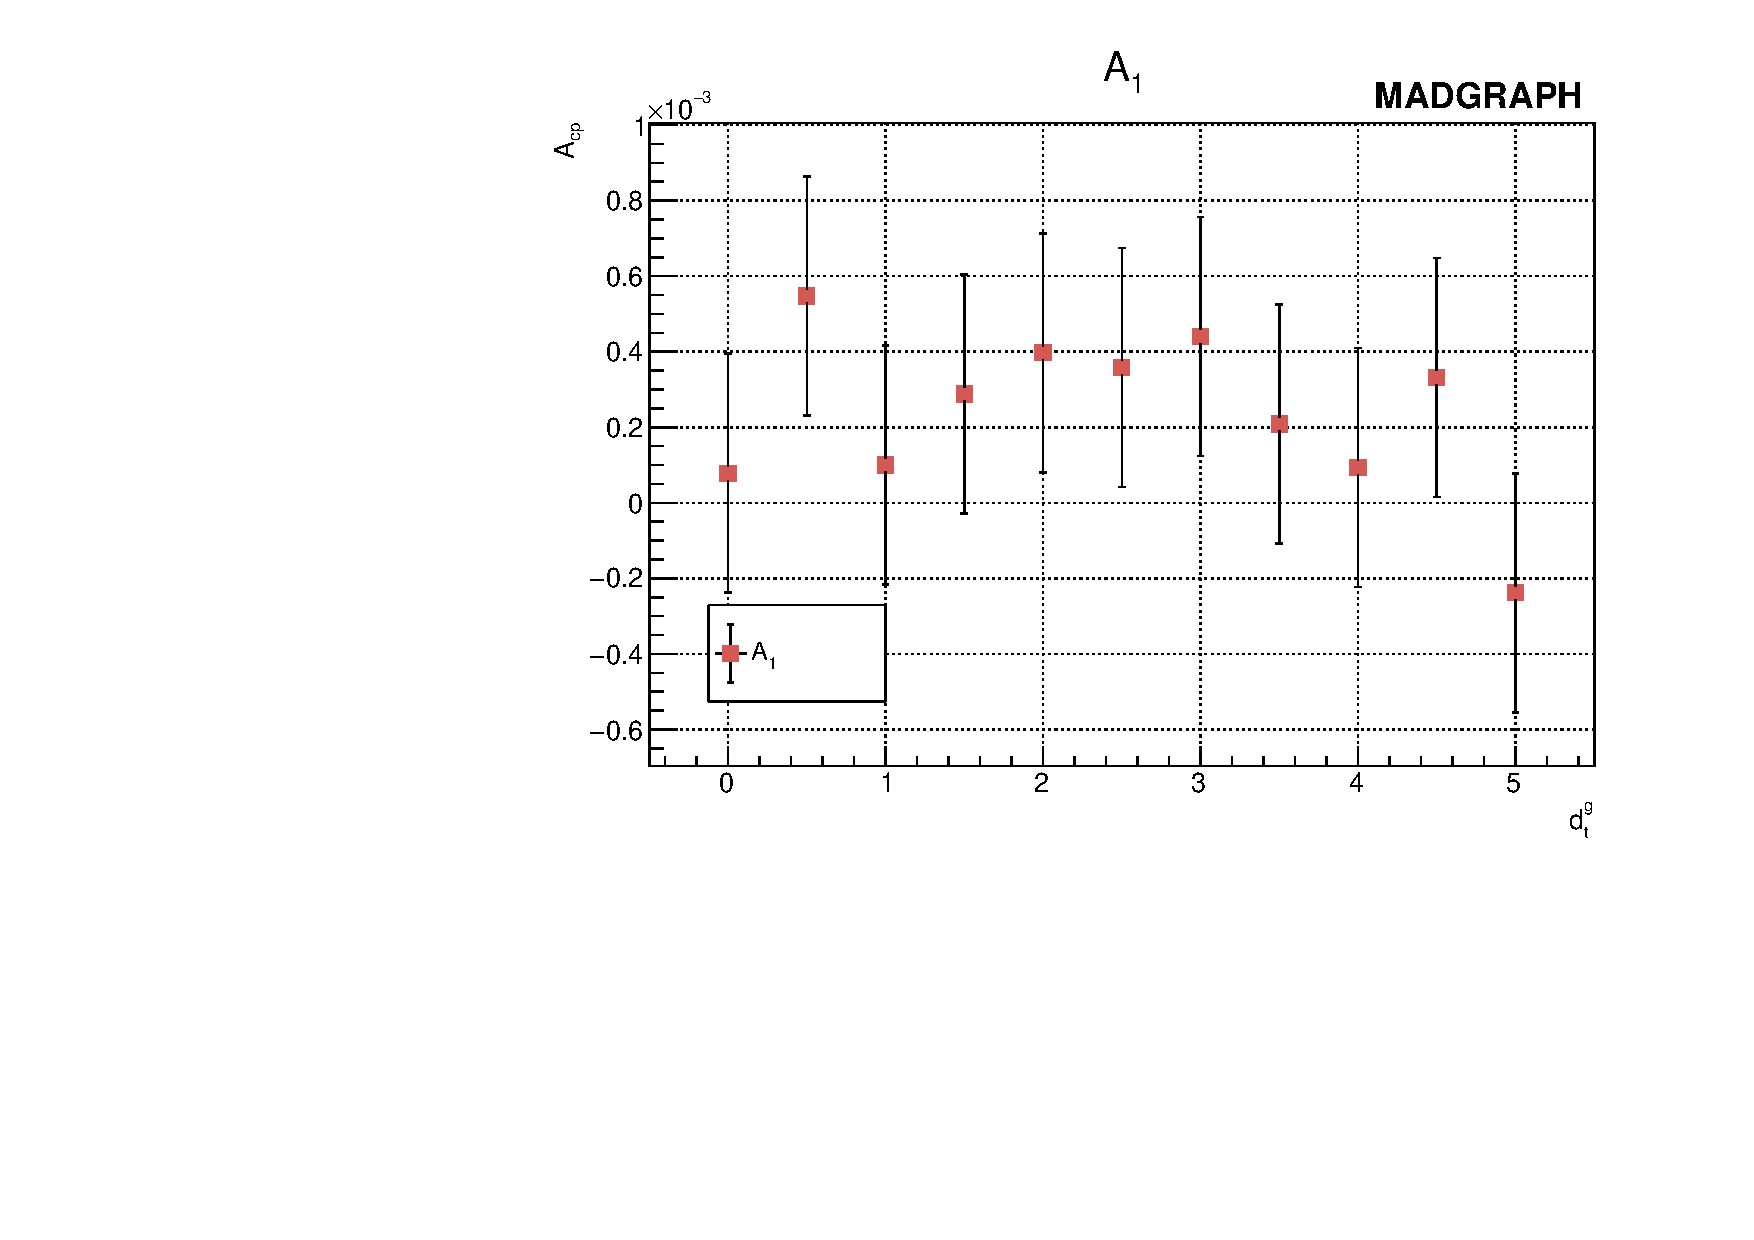
\includegraphics[width=0.45\textwidth]{Figures/Observables/1993/ci_10_7-dilep_0j_NoSel_B1993_A1.pdf}}
			    \subfigure[$A_2$]{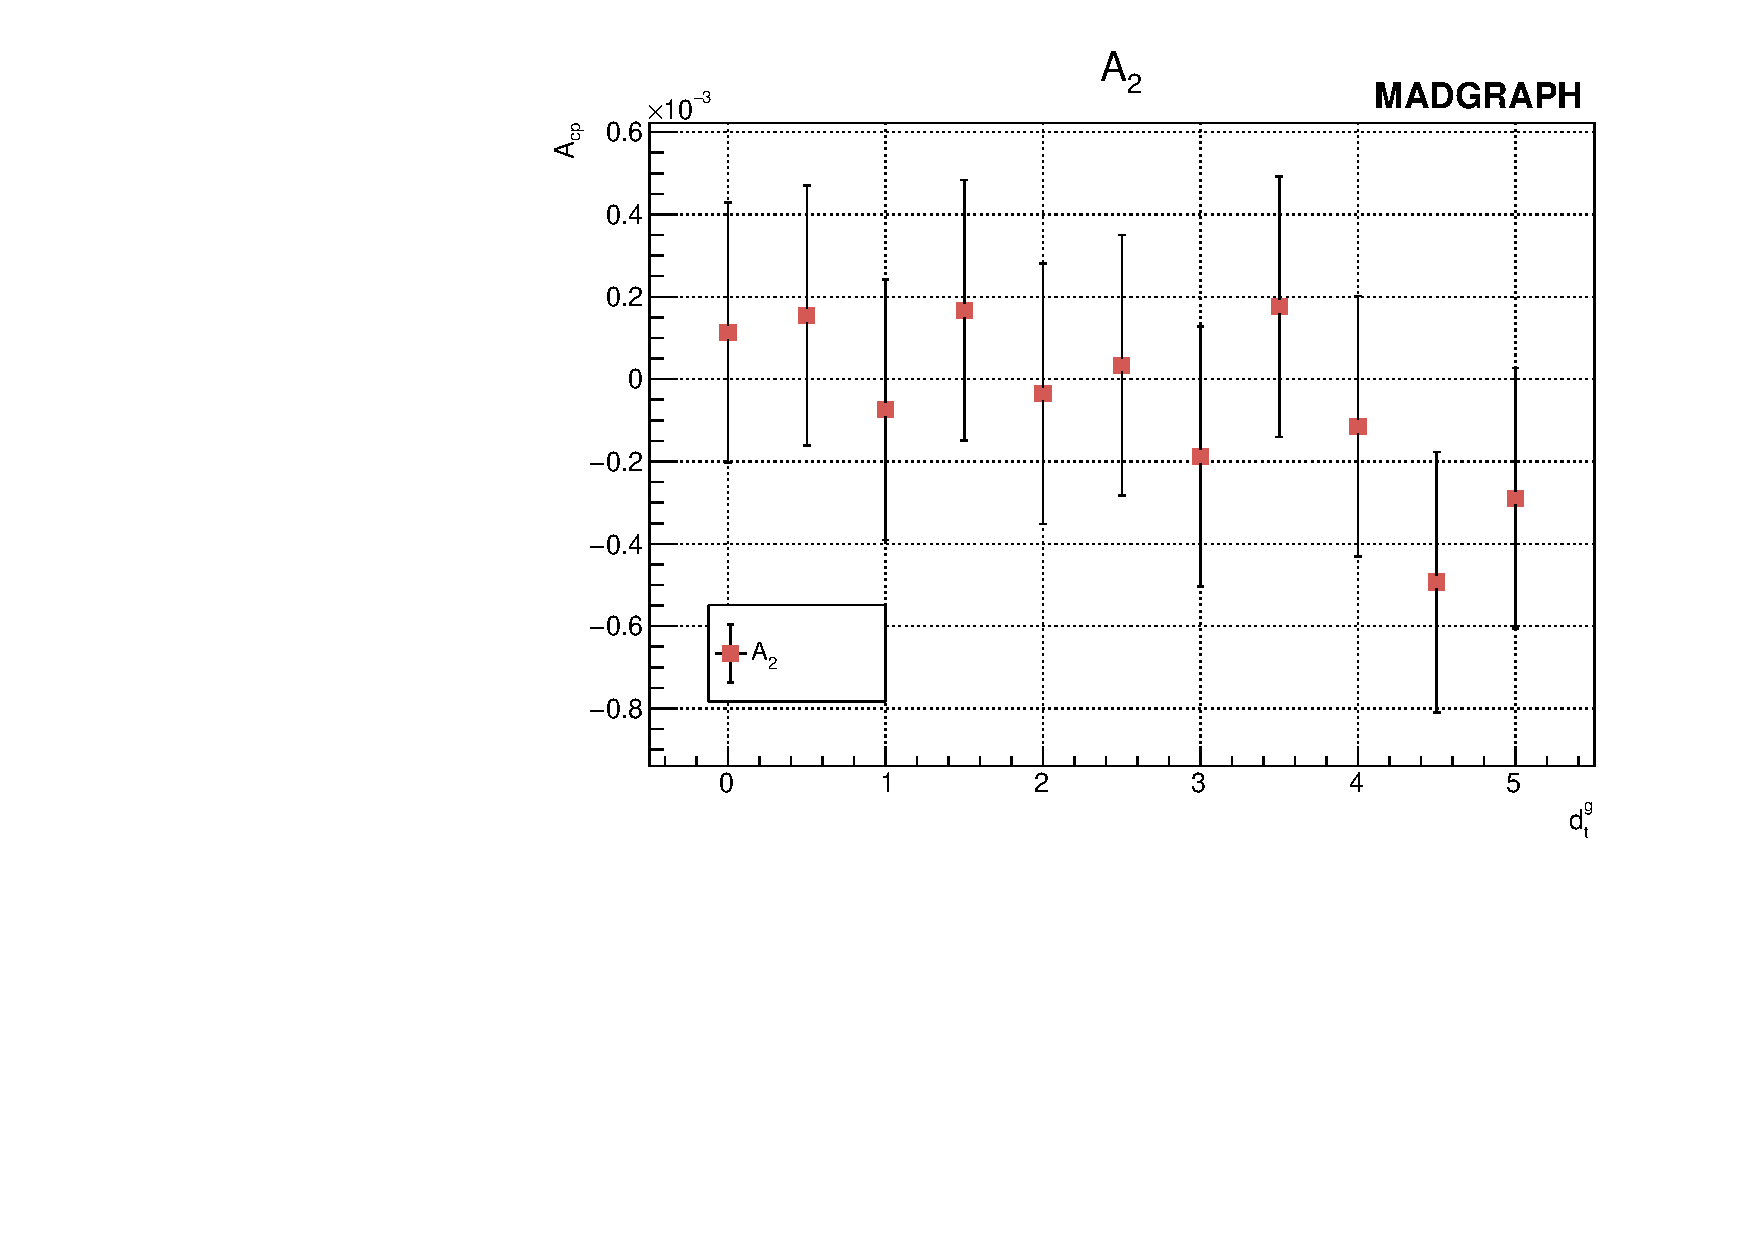
\includegraphics[width=0.45\textwidth]{Figures/Observables/1993/ci_10_7-semi_0j_NoSel_B1993_A2.pdf}}\\
			\caption{CEDM model $t\bar{t}$ sample under $A_1$ and $A_2$ observables ($d_t^g$ = 0-5, $10^7$ dilepton/semi-leptonic $t\bar{t}$ events w/o selection)}
			\label{Obs:fig:CEDM_1993}
			\end{figure}
			\FloatBarrier

			\begin{figure}[H]
			\centering
				\subfigure[$A_{cp}(Q_1)$]{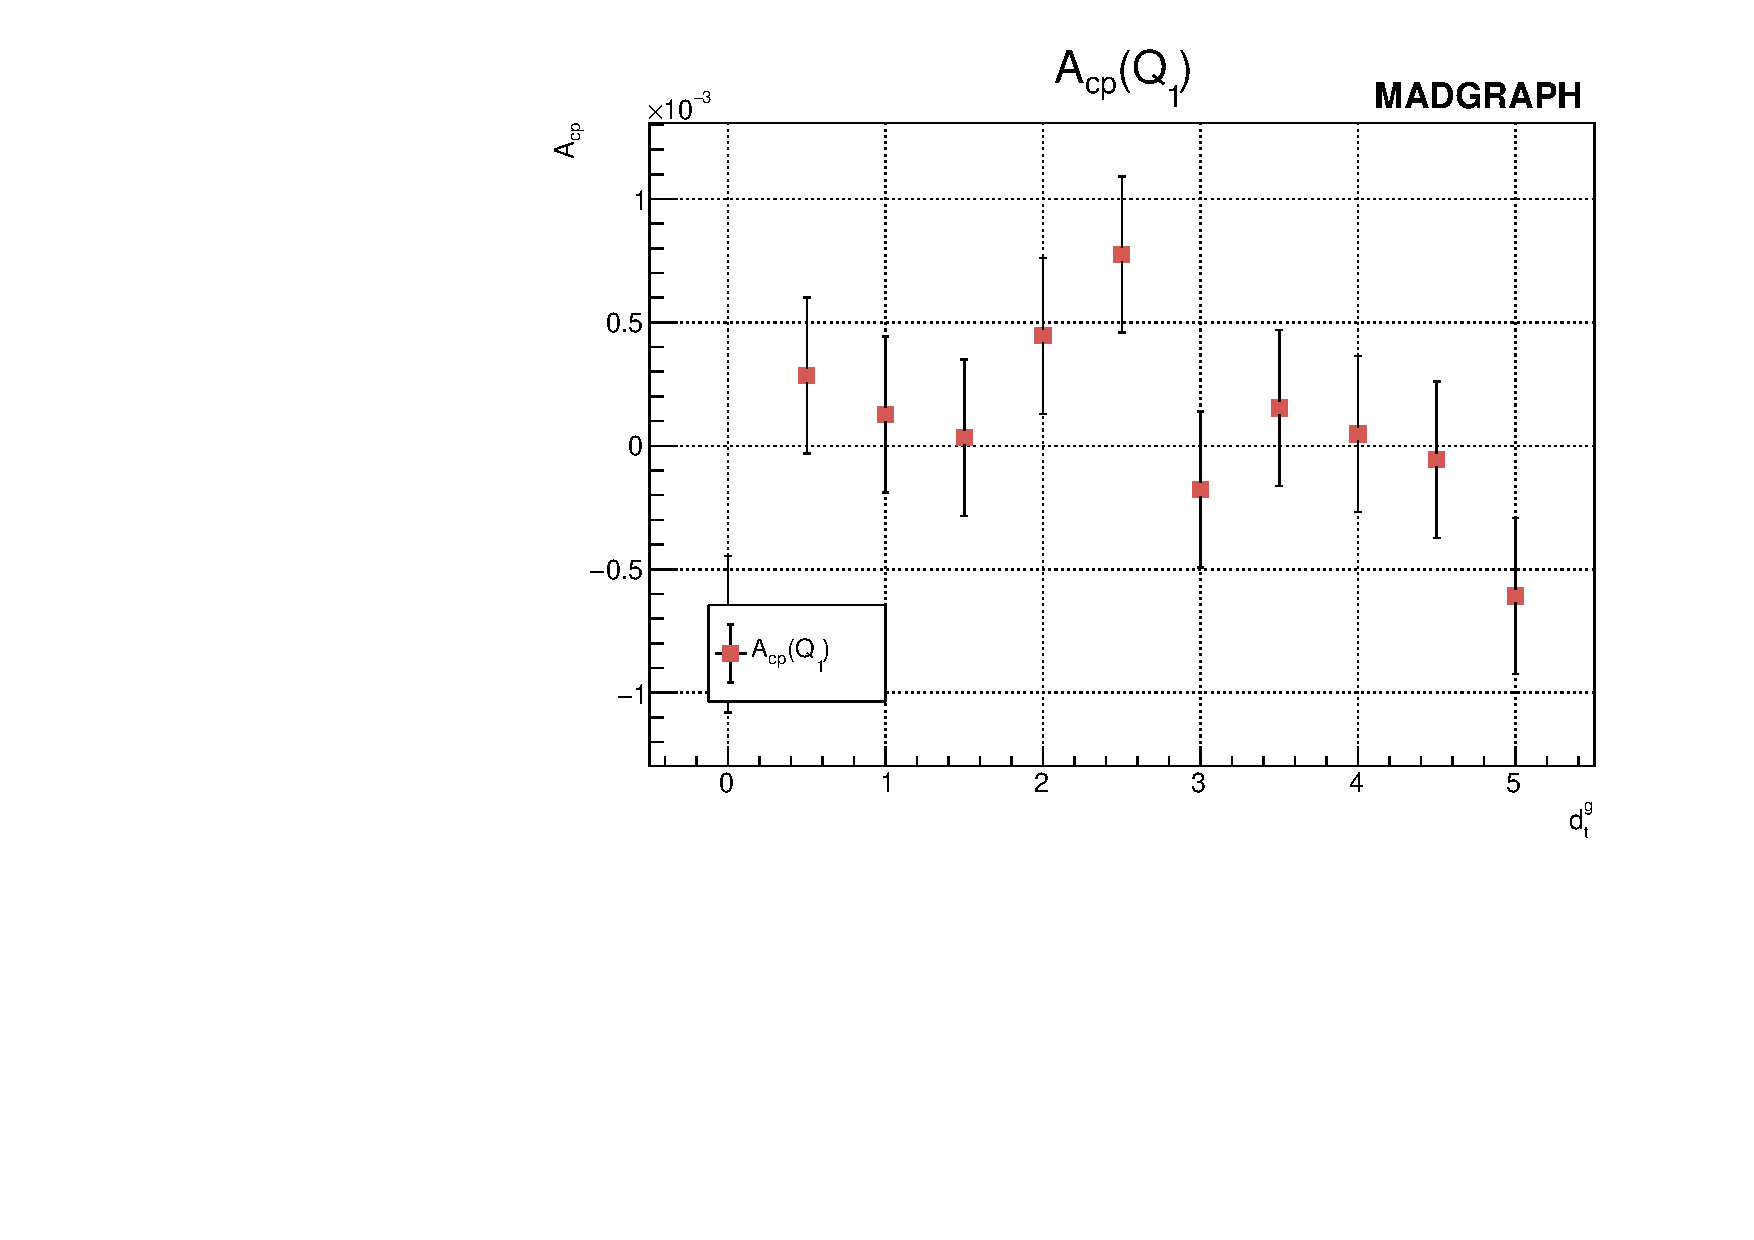
\includegraphics[width=0.45\textwidth]{Figures/Observables/1998/ci_10_7-dilep_0j_NoSel_B1998_Q1.pdf}}
			    \subfigure[$A_{cp}(O_1)$]{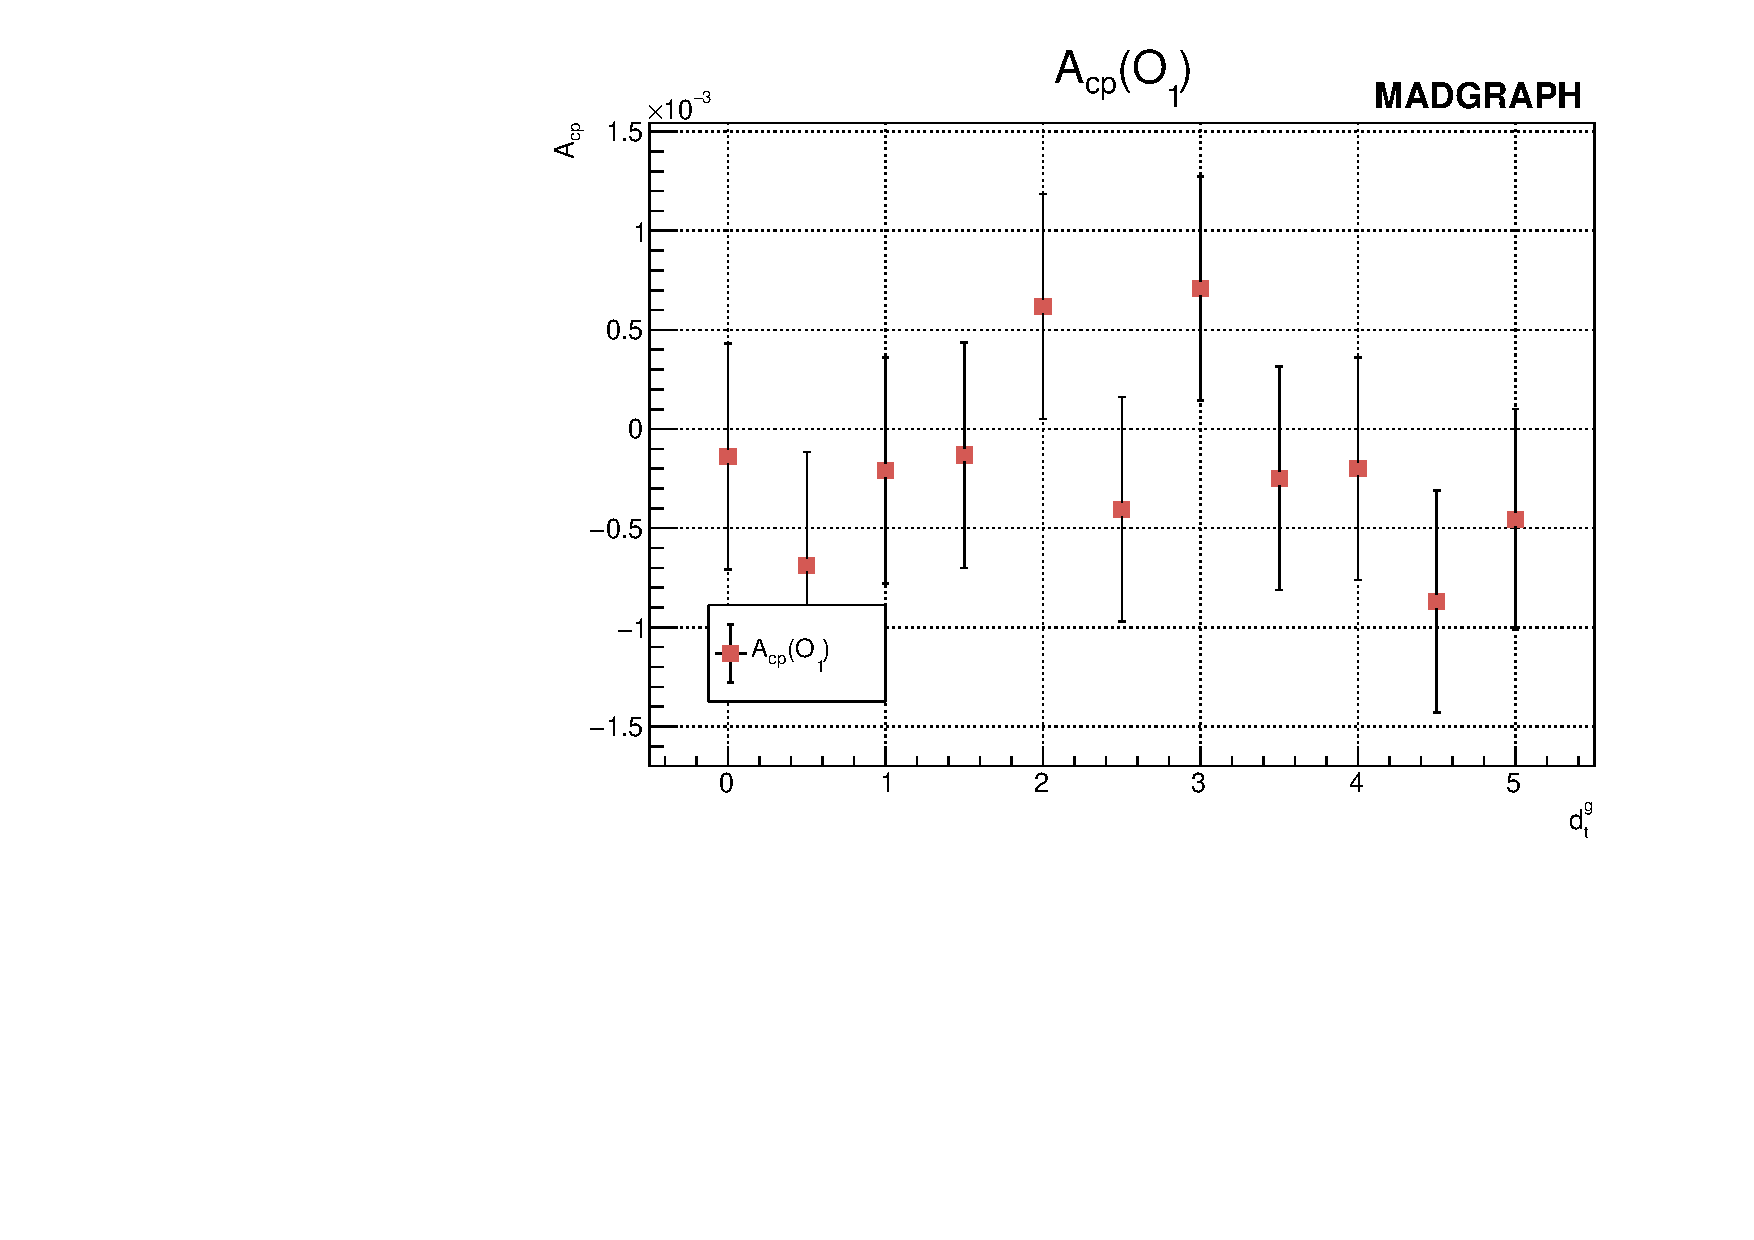
\includegraphics[width=0.45\textwidth]{Figures/Observables/1998/ci_10_7-semi_0j_NoSel_B1998_O1.pdf}}\\
			\caption{CEDM model $t\bar{t}$ sample under $A_{cp}(Q_1)$ and $A_{cp}(O_1)$, observables ($d_t^g$ = 0-5, $10^7$ dilepton/semi-leptonic $t\bar{t}$ events w/o selection)}
			\label{Obs:fig:CEDM_1998}
			\end{figure}
			\FloatBarrier

			As our expectation, there is no obvious sensitivity in Fig.\ref{Obs:fig:CEDM_1993} and \ref{Obs:fig:CEDM_1998} to detect real part of $d_t^g$ by T-even observables. However, we can focus on SM and 2HDM with these 4 T-even observables, there are the test with $10^7$ events $t\bar{t}$ dilepton/semi-leptonic sample(w/o selection), by SM and 2HDM default parameter setting:

			\begin{figure}[H]
			\centering
				\subfigure[$A_1$]{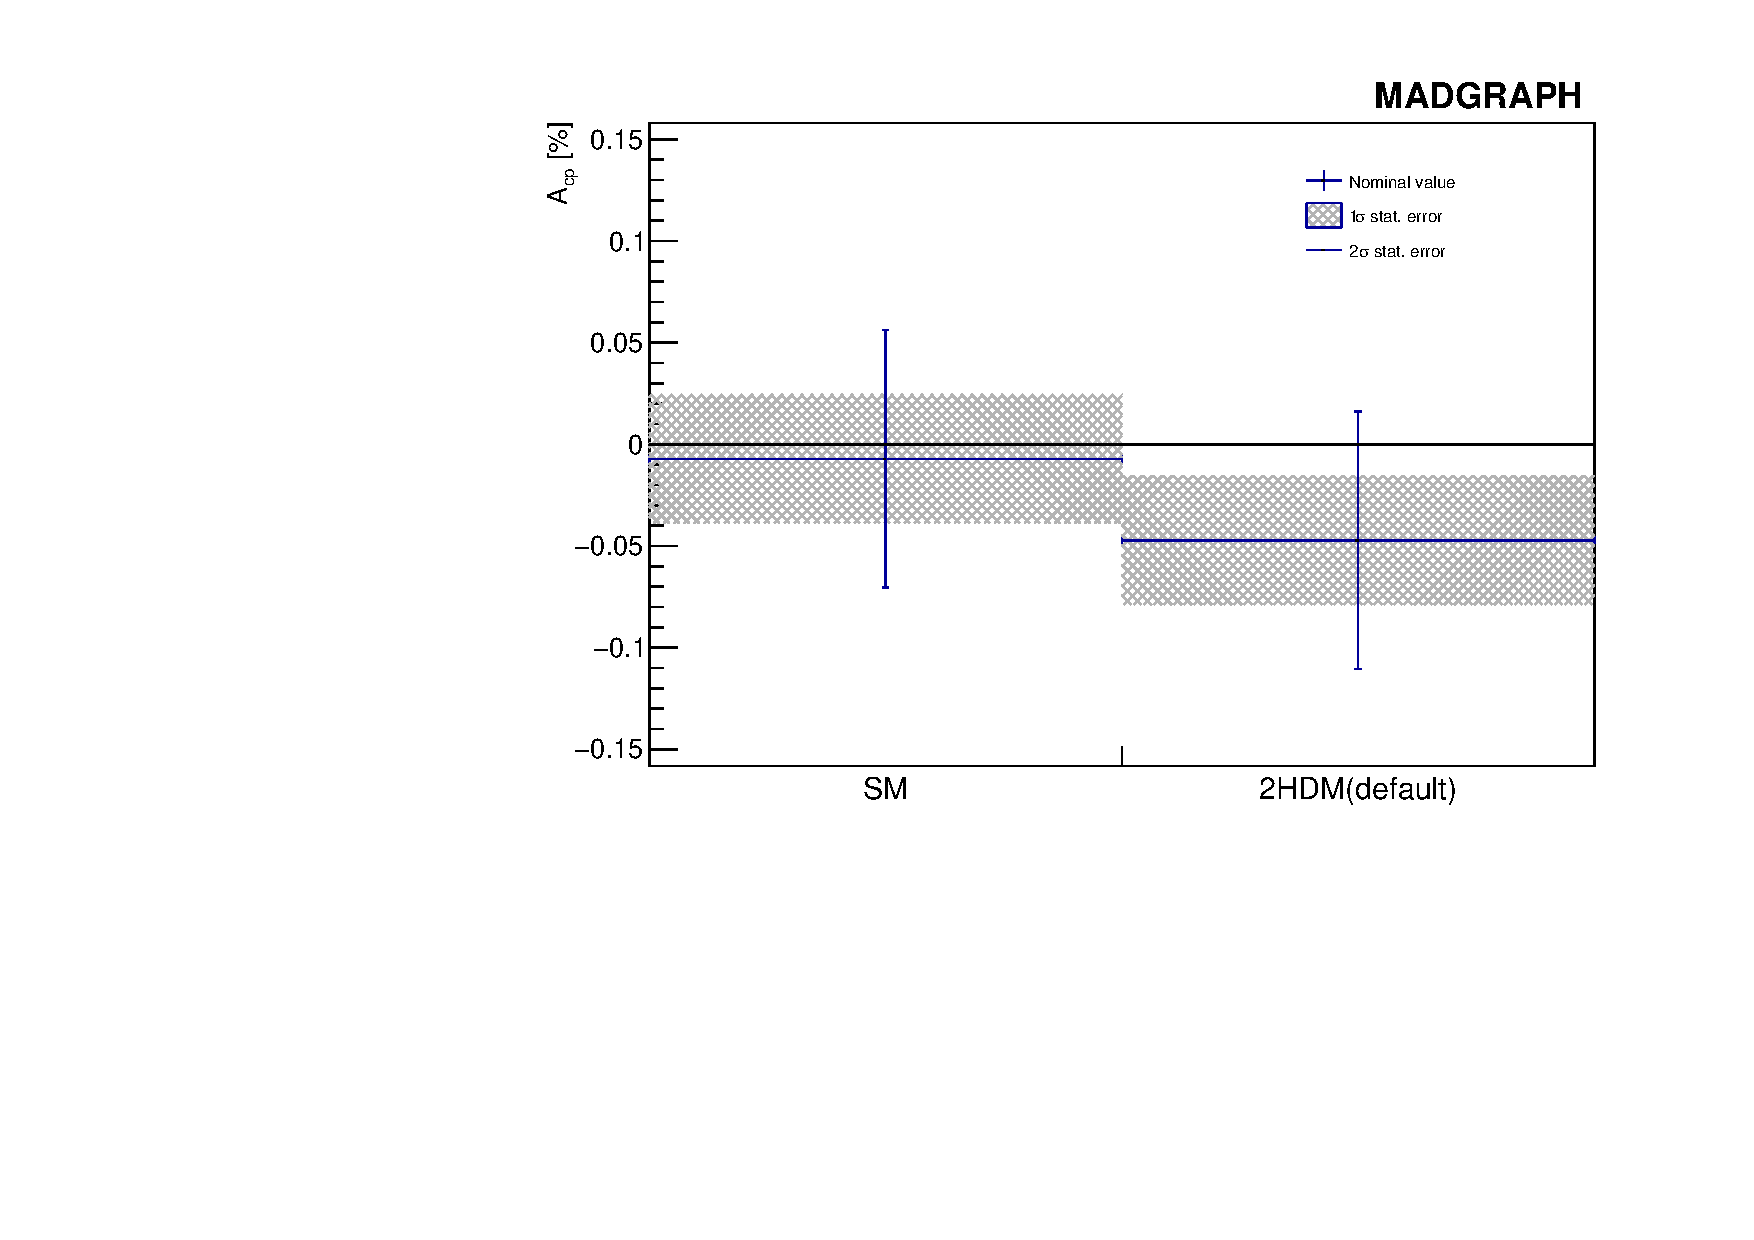
\includegraphics[width=0.45\textwidth]{Figures/Observables/1993/Graph_2HDM_default_B1993_A1_NoSel_new.pdf}}
			    \subfigure[$A_2$]{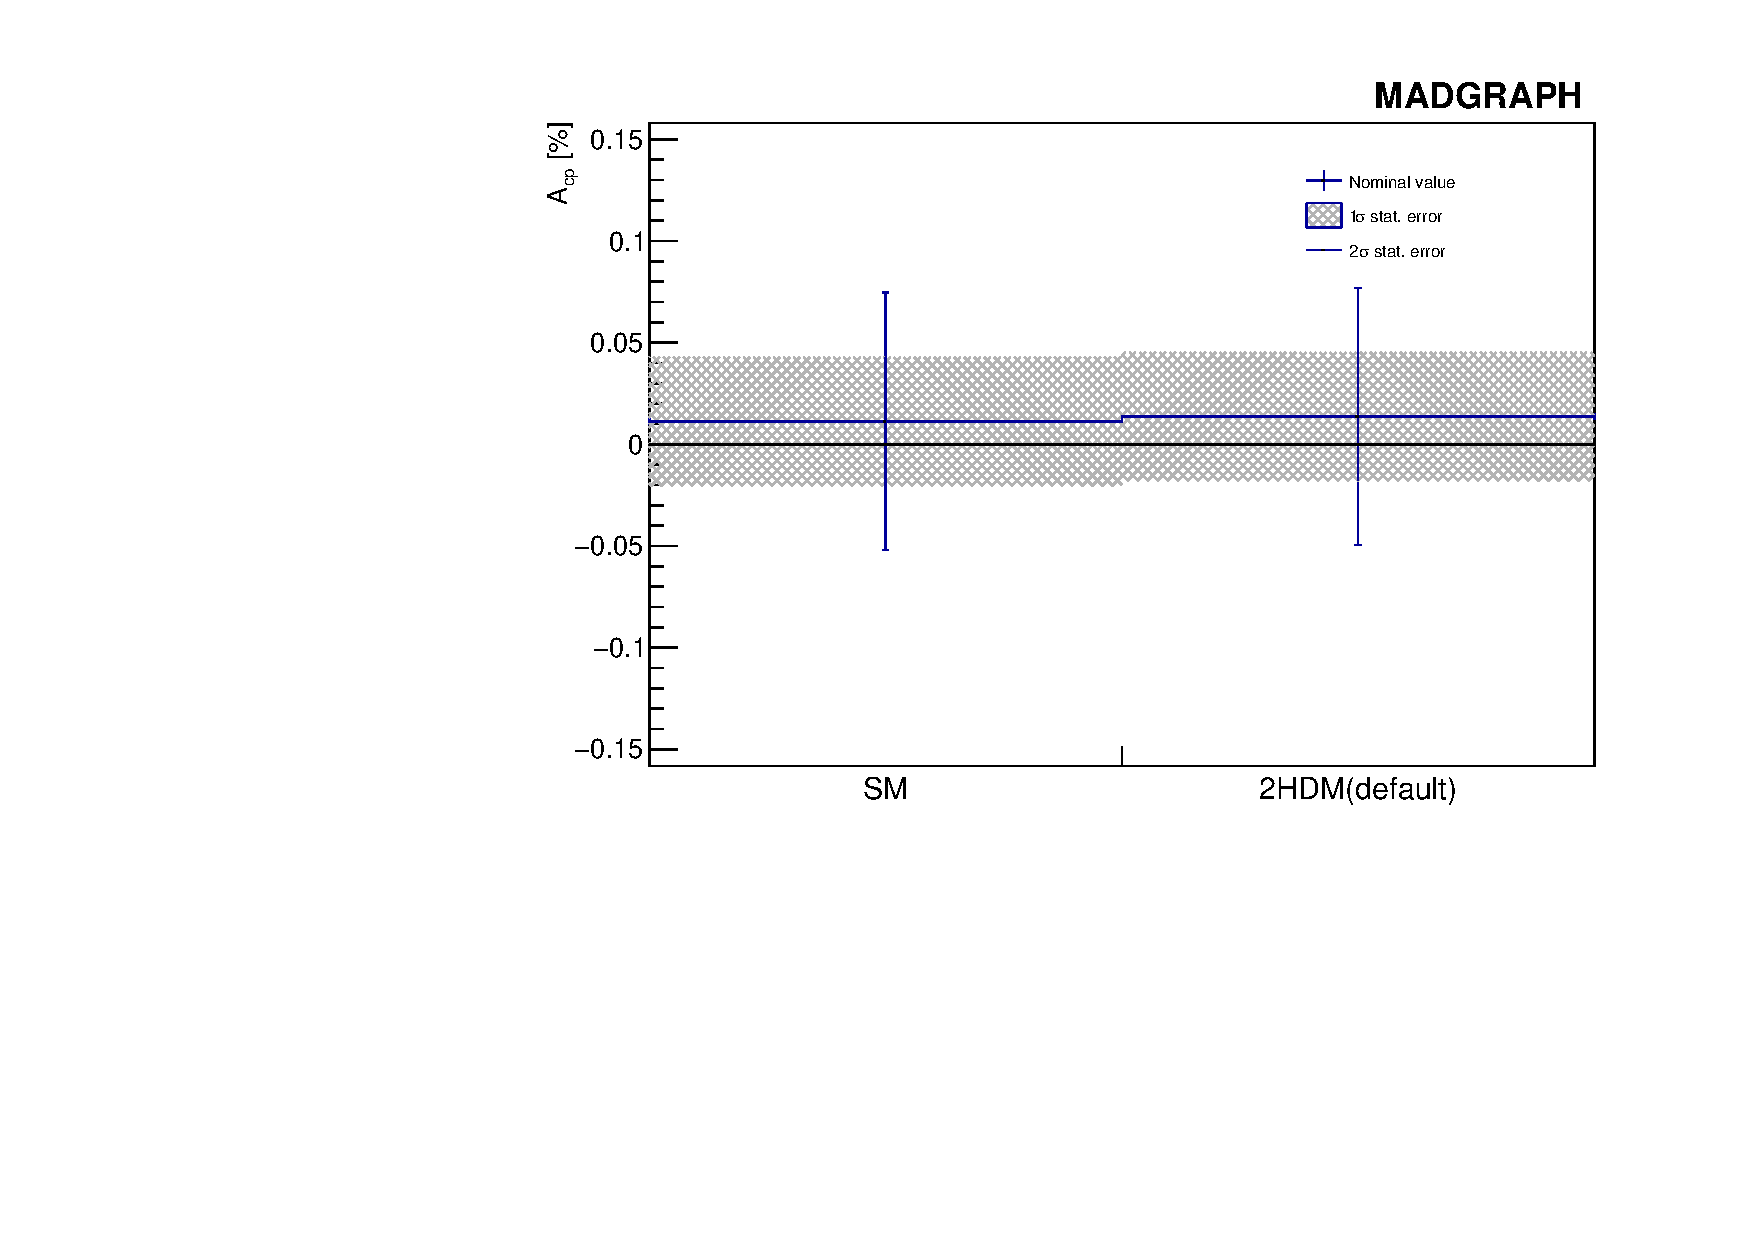
\includegraphics[width=0.45\textwidth]{Figures/Observables/1993/Graph_2HDM_default_B1993_A2_NoSel_new.pdf}}\\
			\caption{SM, 2HDM(default) sample measured by $A_1$, $A_2$}
			\label{Obs:fig:SM_2HDM_1993}
			\end{figure}
			\FloatBarrier

			\begin{figure}[H]
			\centering
				\subfigure[$A_{cp}(Q_1)$]{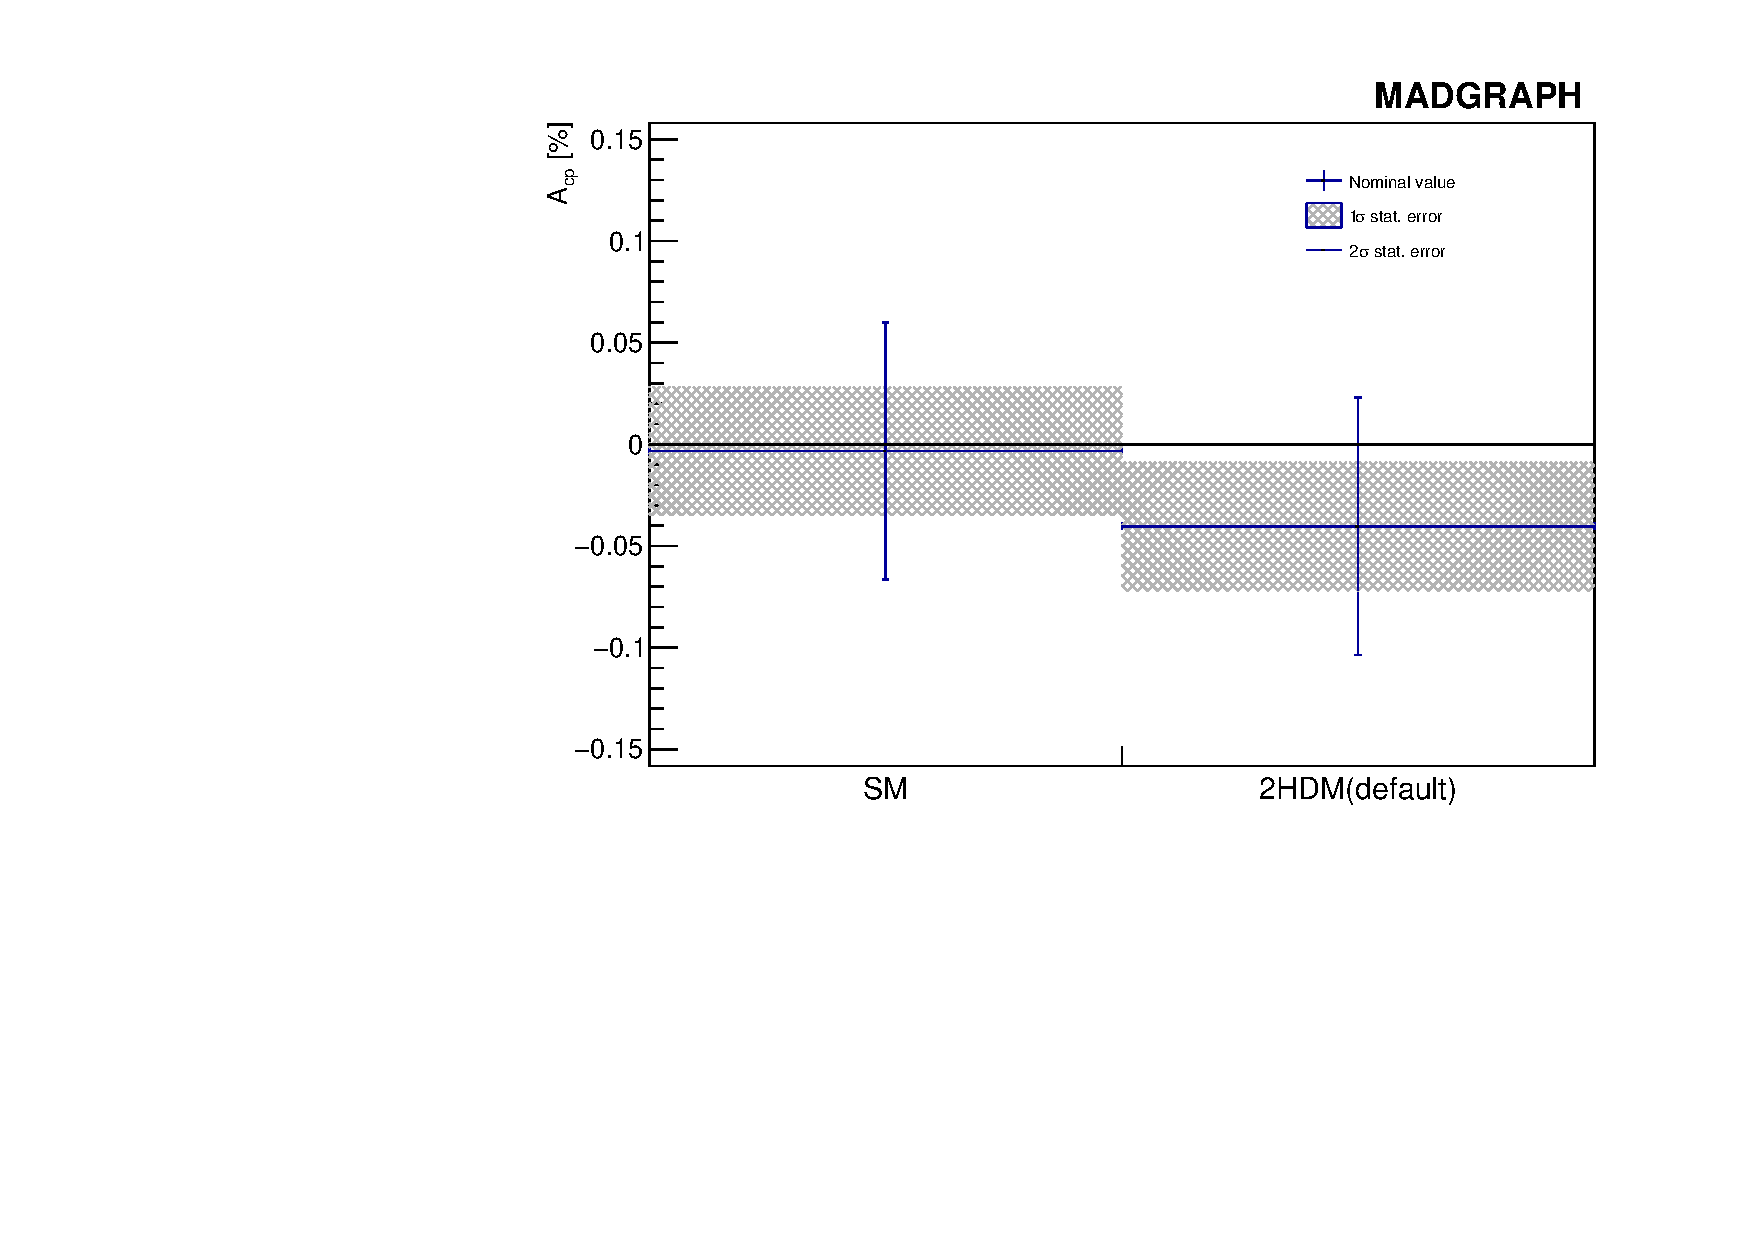
\includegraphics[width=0.45\textwidth]{Figures/Observables/1998/Graph_2HDM_default_B1993_Q1_NoSel_new.pdf}}
			    \subfigure[$A_{cp}(O_1)$]{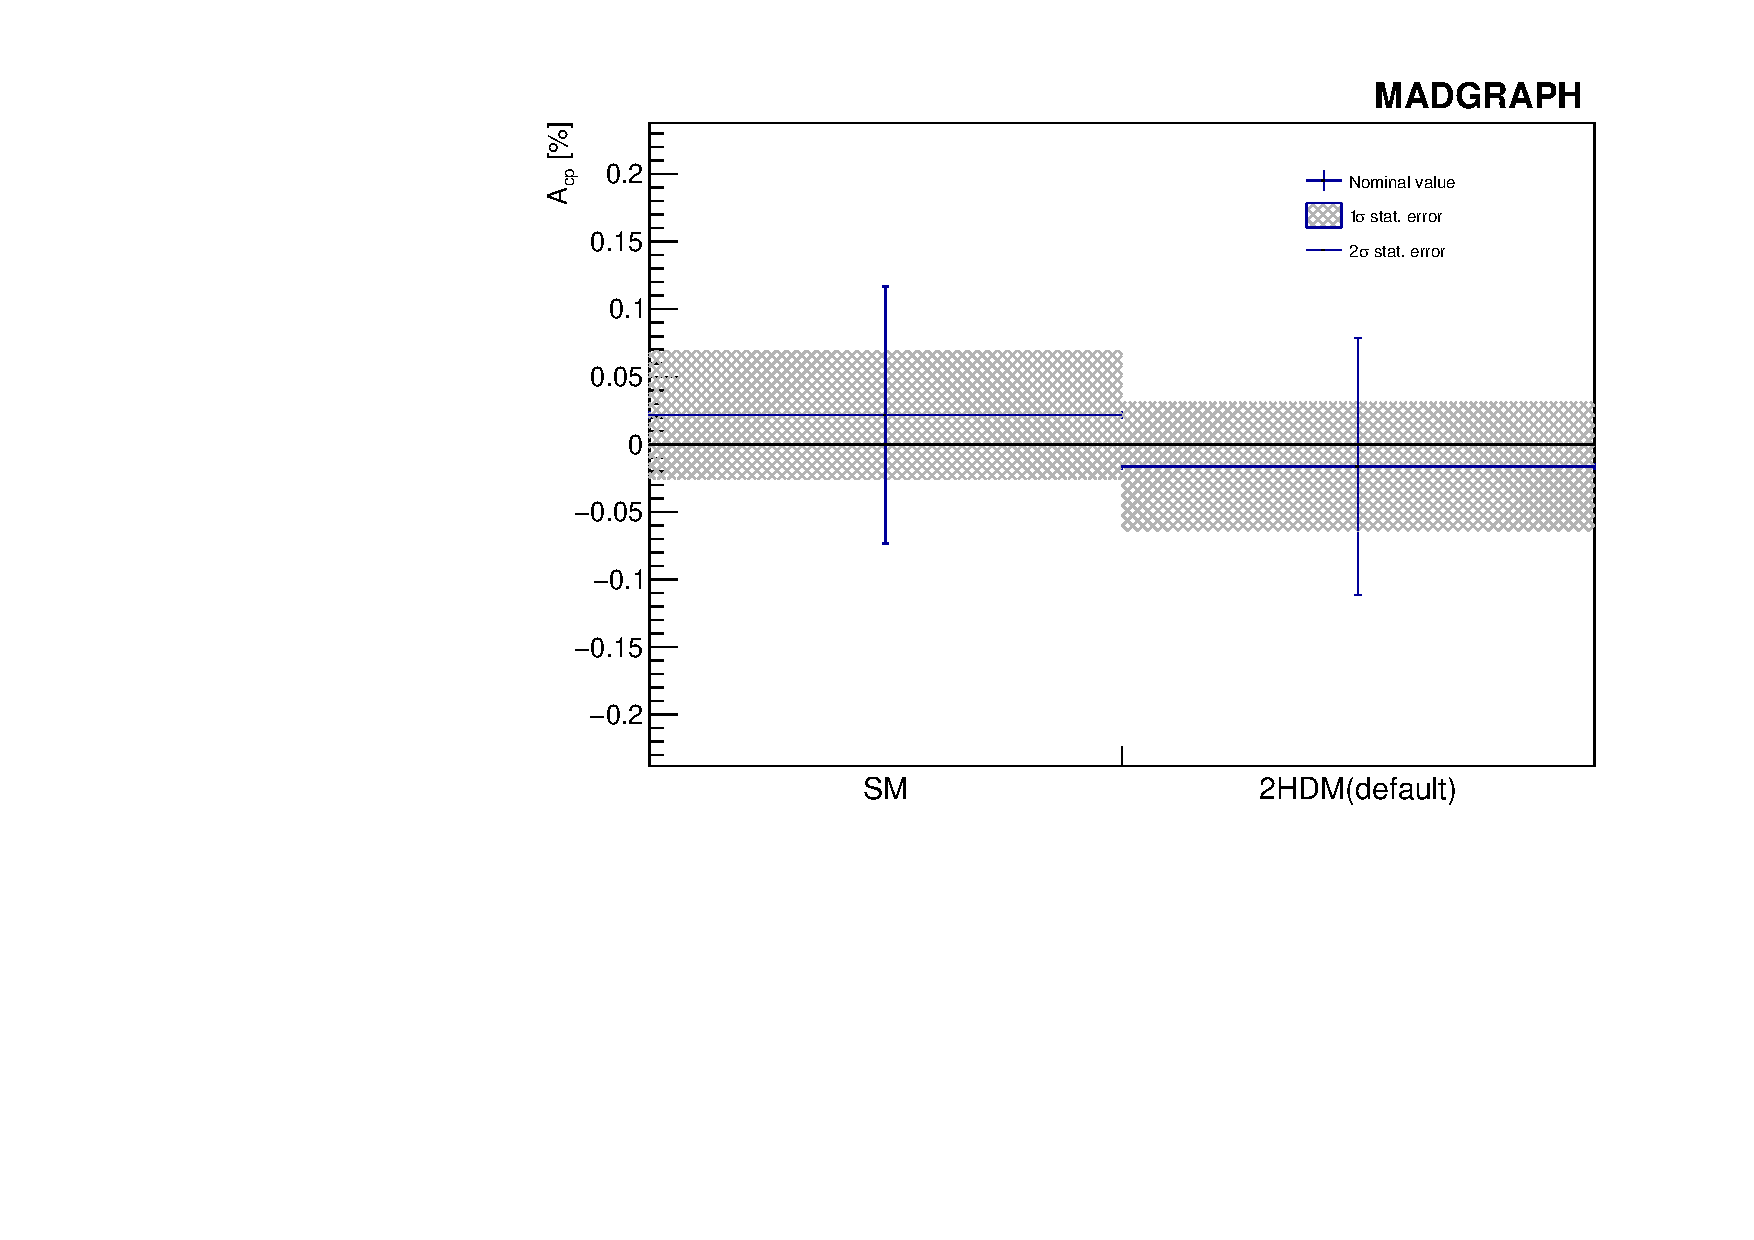
\includegraphics[width=0.45\textwidth]{Figures/Observables/1998/Graph_2HDM_default_B1993_O1_NoSel_new.pdf}}\\
			\caption{SM, 2HDM(default) sample measured by $A_{cp}(Q_1)$, $A_{cp}(O_1)$}
			\label{Obs:fig:SM_2HDM_1998}
			\end{figure}
			\FloatBarrier

			In Fig.\ref{Obs:fig:SM_2HDM_1993} and Fig.\ref{Obs:fig:SM_2HDM_1998}, although the 2HDM looks having more asymmetry than SM sometimes as expected, they are both inside the 2 standard deviation range. I think that would be the fluctuaction and not really present that the observables detect some asymmetry. It is not sure that the parameter setting of 2HDM can not lead to CP violation or the observables have bad sensitivity. The parameter setting of 2HDM is not our business, so the temperal conclusion of observables $A_1$, $A_2$, $A_{cp}(O_1)$, and $A_{cp}(Q_1)$ are that they are detectable, and if there are some exact samples with obvious CPV could be detect by T-even observables, it is valuable to test the observables' sensitivity about CPV. The work we can do now is to do the research of these observables themselves and their properties.

		\subsubsection{Observable property}
		\label{sssec:AcpObs_property}

			In this section, we focus on the dilution effect of T-evenn observables. However, the previous T-even observables' forms are various, the appropriate observables which can be done with studying dilution effect are $A_{cp}(Q_1)$ and $A_{cp}(O_1)$ because of their counting the positive and negative events number rather than measuring observable's value, that is to say, they are just like the method the 2016 analysis uses with the four T-odd observables($O_3$, $O_6$, $O_{12}$, $O_{14}$). Eq.********(in chapter 1)

			To see the dilution effects, we need the simulation not only in parton level with Madgraph, but also in showering and detector level objects' simulation with Pythia and Delphes. The concept of dilution effect here is same as section.\ref{sec:Dilution} -- the effect which dilutes the $A_{cp}$ in generator-level to $A'_{cp}$ in detector-level. However, the test here is using generator-matching to match detector-level's objects and generator-level's particles, so the measured result would be purely from detector/reconstruction issue and objects' resolution, not from objects' identification like b-tagged correctness, light jets' identification. The generator-matching has been mentioned in section.\ref{sssec:mva_intro}, and the matching method is by Eq.\ref{eq:gen_matching}.

			With the same calculation method, we also use Eq.\ref{eq:Dilution_epsilon} to calculate the dilution factor of $A_{cp}(Q_1)$ and $A_{cp}(O_1)$ by SM $t\bar{t}$ simulation sample with no selection($10^7$ events):

			\begin{center}
			\setlength{\tabcolsep}{12pt}
			\begin{longtable}{ c | c c }
			\caption{Dilution factor of }\\
			Observable & same sign rate[\%]($=1-\epsilon_{opp}$) & Dilution Factor[\%] \\
			\hline
			$A_{cp}(Q_1)$ & 88.12  &  76.23  \\
			$A_{cp}(O_1)$    &    \\
			\hline
			\end{longtable}
			\label{Obs:tb:SM_DF}
			\end{center}

			We can validate the dilution factor by generate samples with artificial $A_{cp}$. The artificial $A_{cp}$ comes from randomly duplicate specific events in original $t\bar{t}$ sample. Take $A_{cp}(Q_1)$ for instance, we have $10\%$ probability to duplicate the $t\bar{t}$ event which has $Q_1 > 0$. There are the validation with varied artificial $A_{cp}$ and their corresponding $A'_{cp}$, then the linearly fitted line's slope would be the dilution factor.(Fig.\ref{Obs:fig:vali_SM})

			\begin{figure}[H]
			\centering
				\subfigure[$A_{cp}(Q_1)$ ($t\bar{t}$ dilepton decay)]{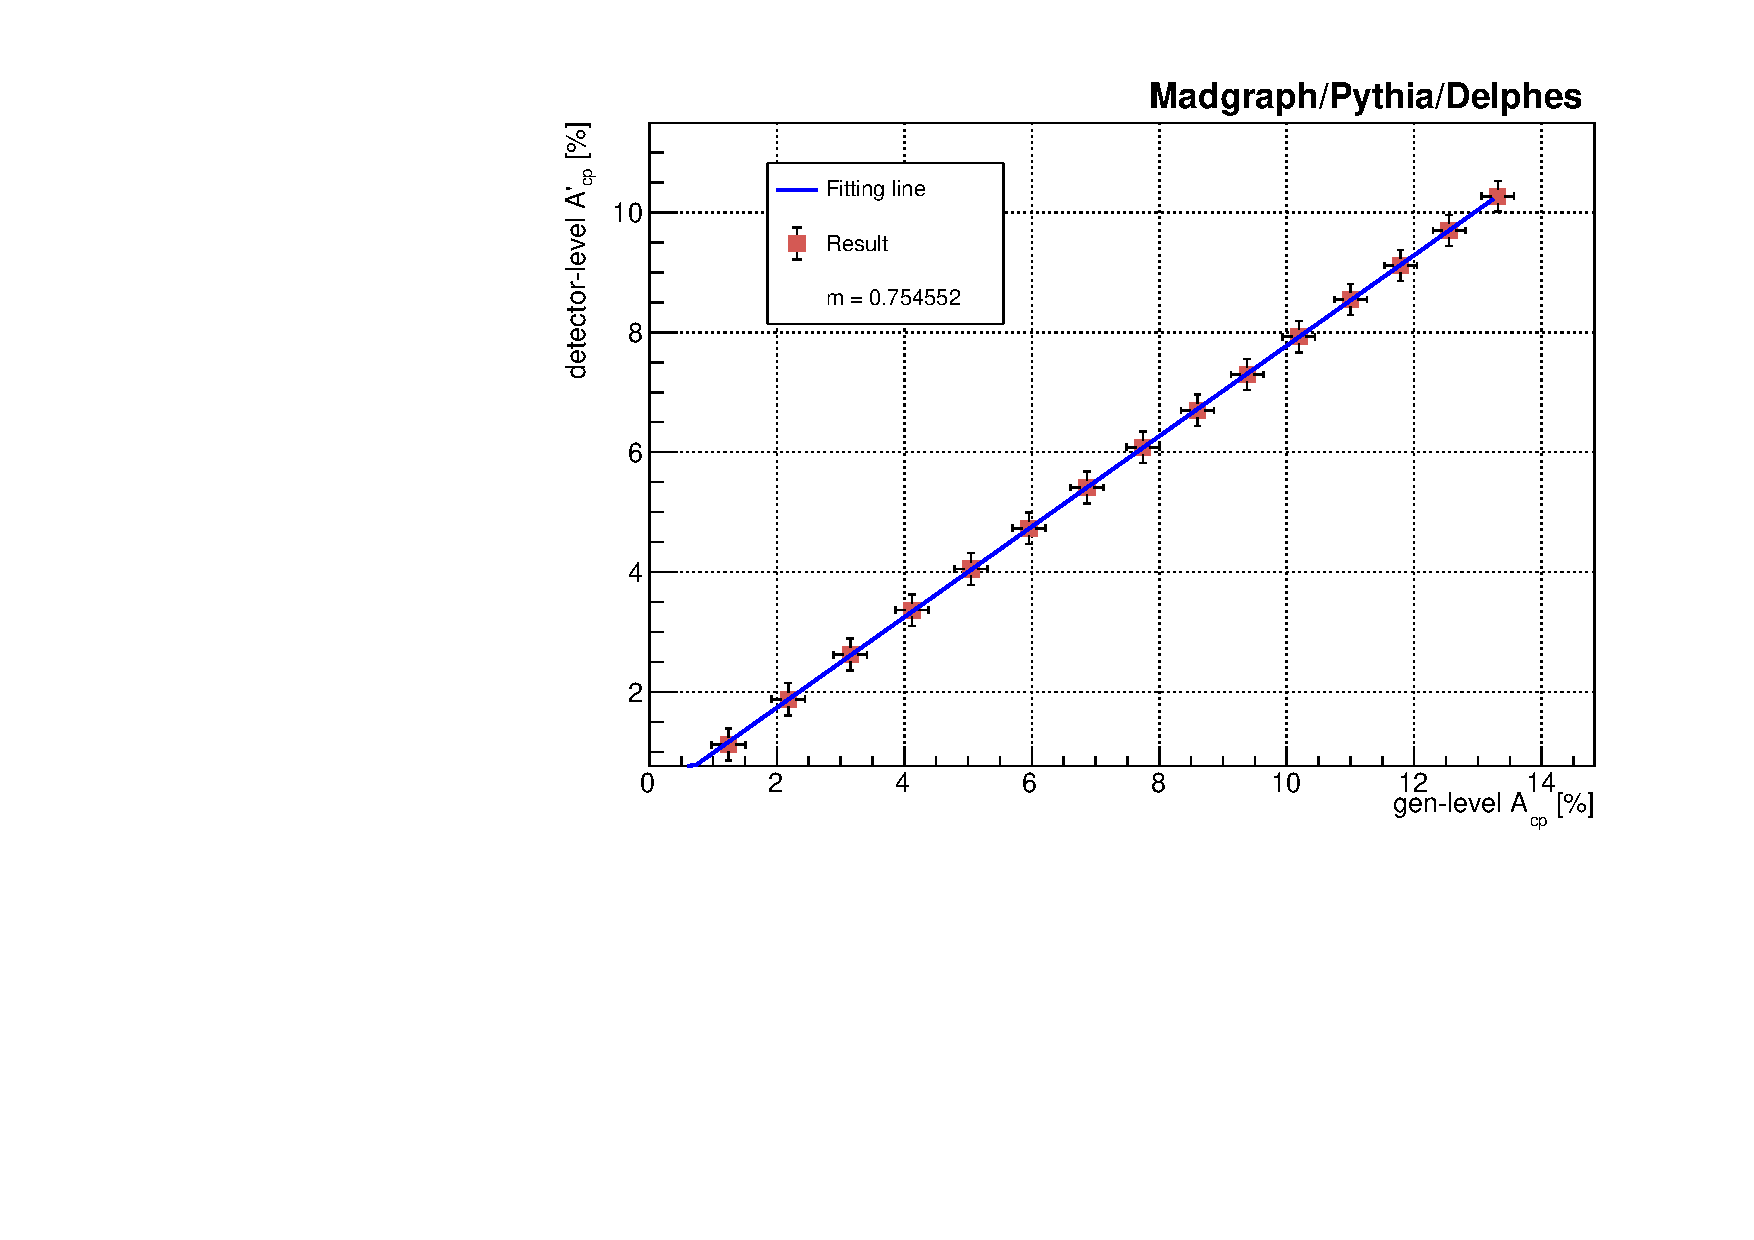
\includegraphics[width=0.45\textwidth]{Figures/Observables/property/text_Dilution_Obs_SM_di_dr.pdf}}
			    \subfigure[$A_{cp}(O_1)$ ($t\bar{t}$ semi-lepton decay)]{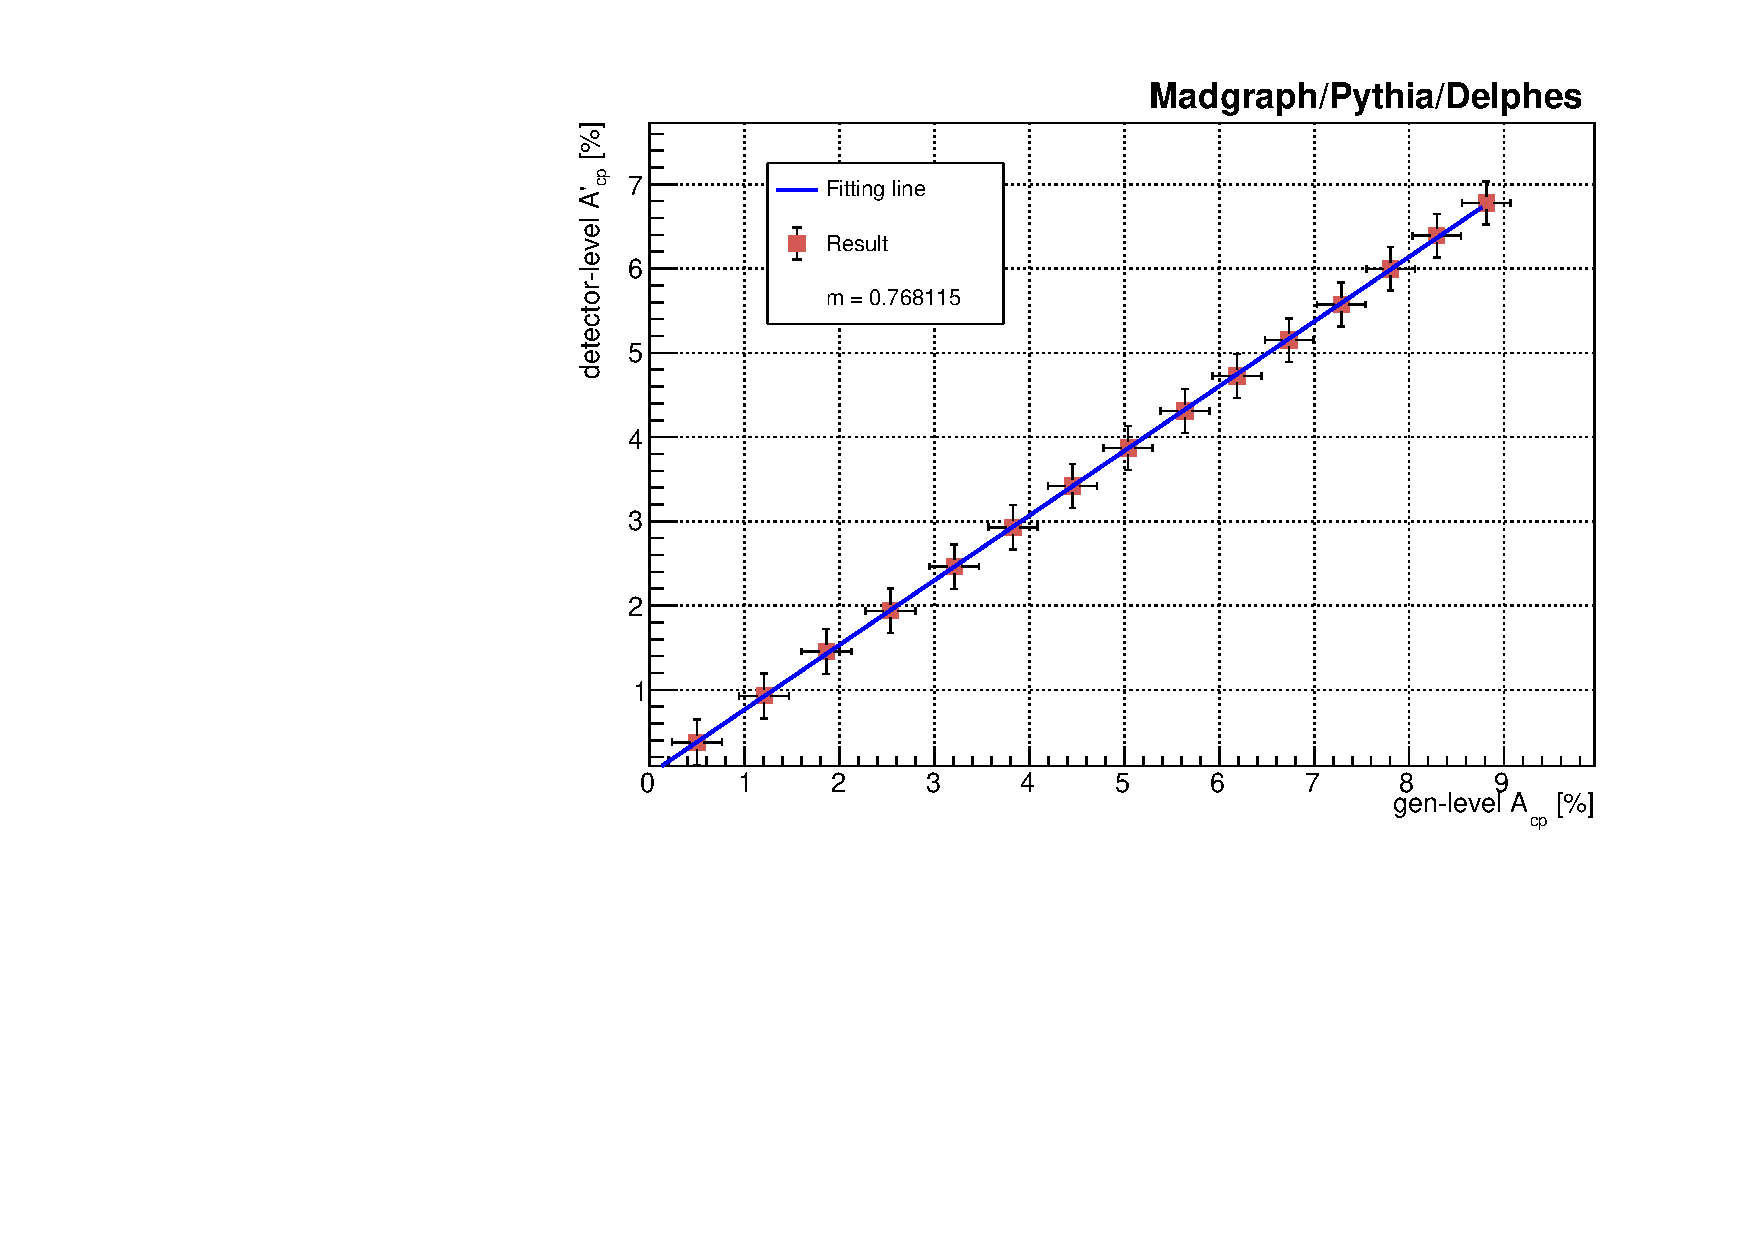
\includegraphics[width=0.45\textwidth]{Figures/Observables/property/text_Dilution_Obs_SM_dr.pdf}}\\
			\caption{Validation of measurred dilution factor with artificial $A_{cp}$'s $t\bar{t}$ simulation samples(SM)}
			\label{Obs:fig:vali_SM}
			\end{figure}
			\FloatBarrier

			The previous measurement of dilution factor is using the standard model's kinematics. However, if we believe the 2HDM sample with default parameter setting has beyond SM's CPV but do not obviously detected by these T-even observables, we may also magnify the CPV in 2HDM model with 2HDM specific kinematics by generate artificial CPV sample. The following are dilution factor calculation and artificial $A_{cp}$'s validation as previous but by 2HDM model(default) $t\bar{t}$ sample:

			\begin{center}
			\setlength{\tabcolsep}{12pt}
			\begin{longtable}{ c | c c }
			\caption{}\\
			Observable & same sign rate[\%]($=1-\epsilon_{opp}$) & Dilution Factor[\%] \\
			\hline
			$A_{cp}(Q_1)$ & 88.30  &  76.61  \\
			$A_{cp}(O_1)$    &    \\
			\hline
			\end{longtable}
			\label{Obs:tb:2HDM_DF}
			\end{center}

			\begin{figure}[H]
			\centering
				\subfigure[$A_{cp}(Q_1)$ ($t\bar{t}$ dilepton decay)]{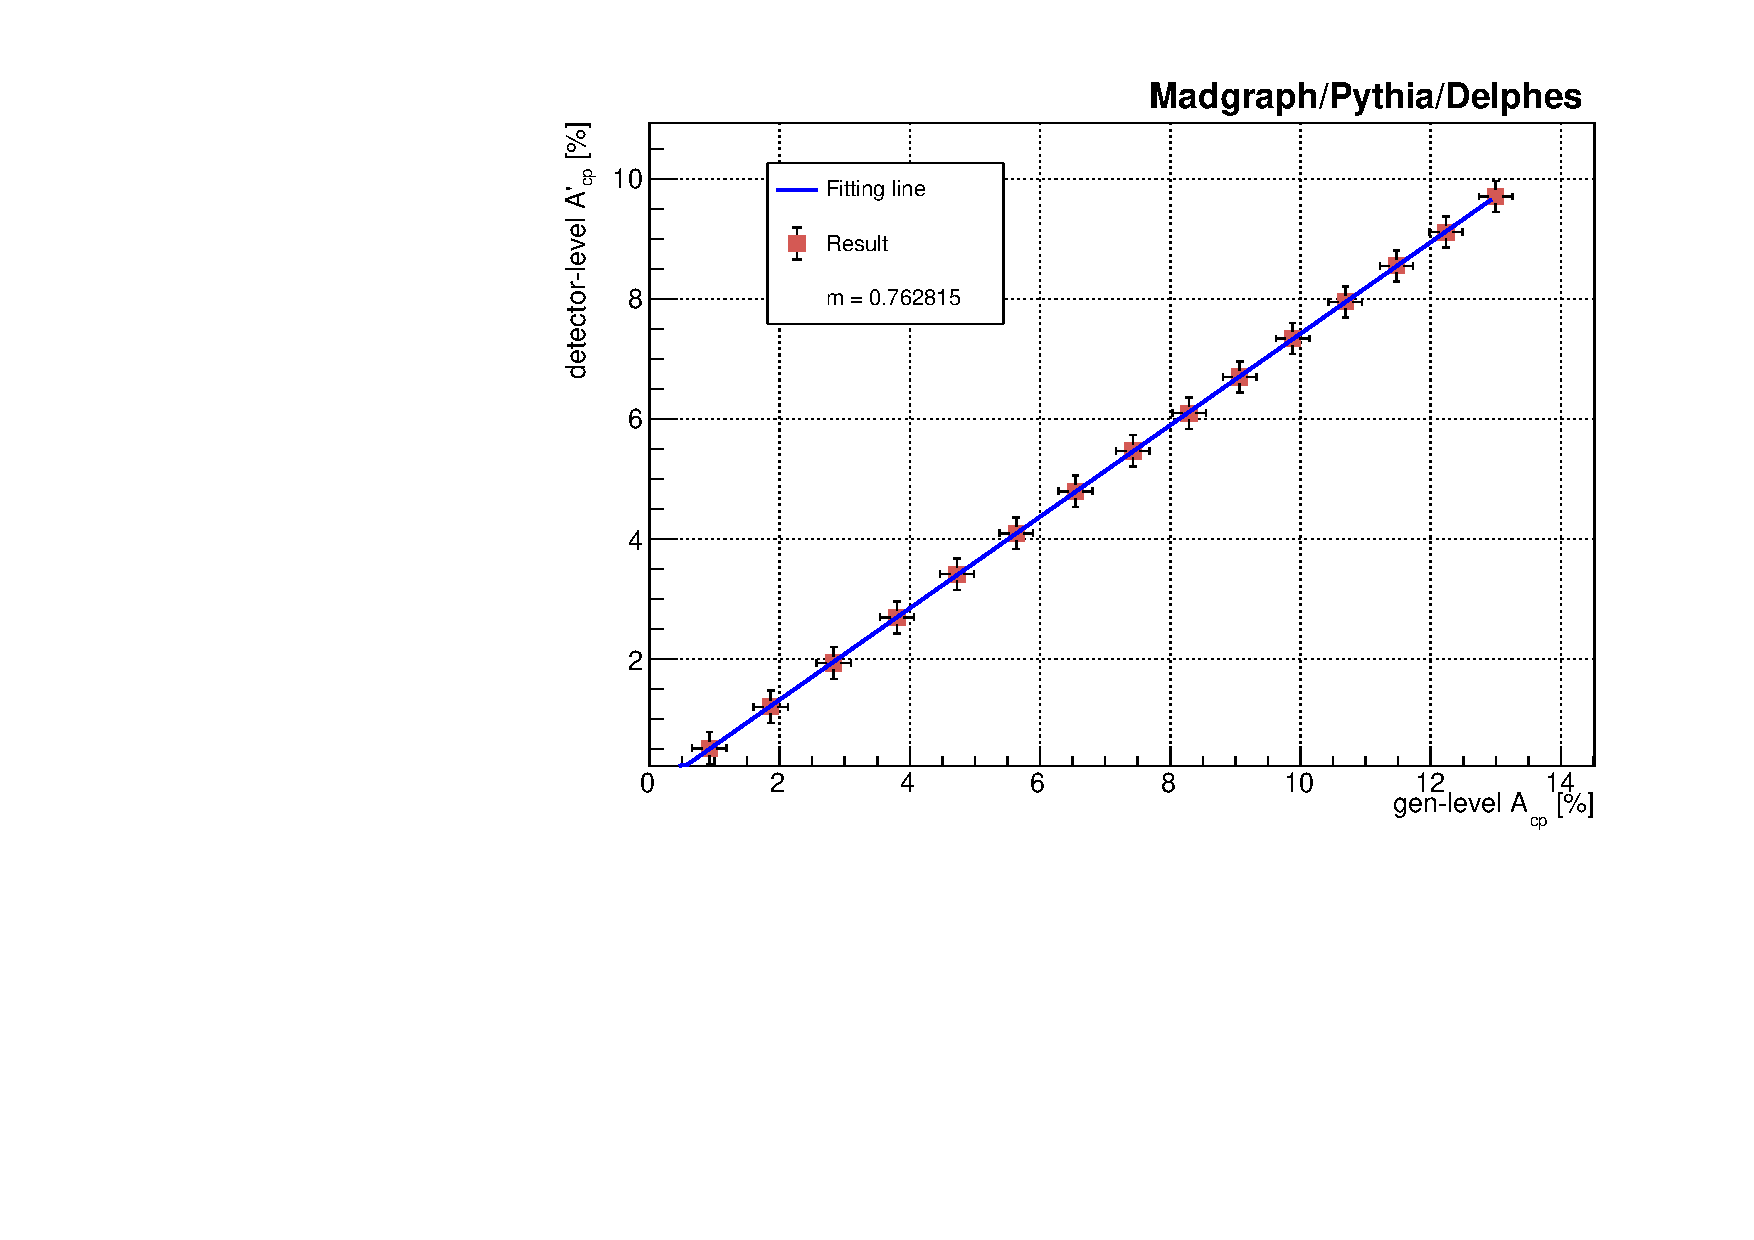
\includegraphics[width=0.45\textwidth]{Figures/Observables/property/text_Dilution_Obs_di_2HDM_NLO_v1_dr.pdf}}
			    \subfigure[$A_{cp}(O_1)$ ($t\bar{t}$ semi-lepton decay)]{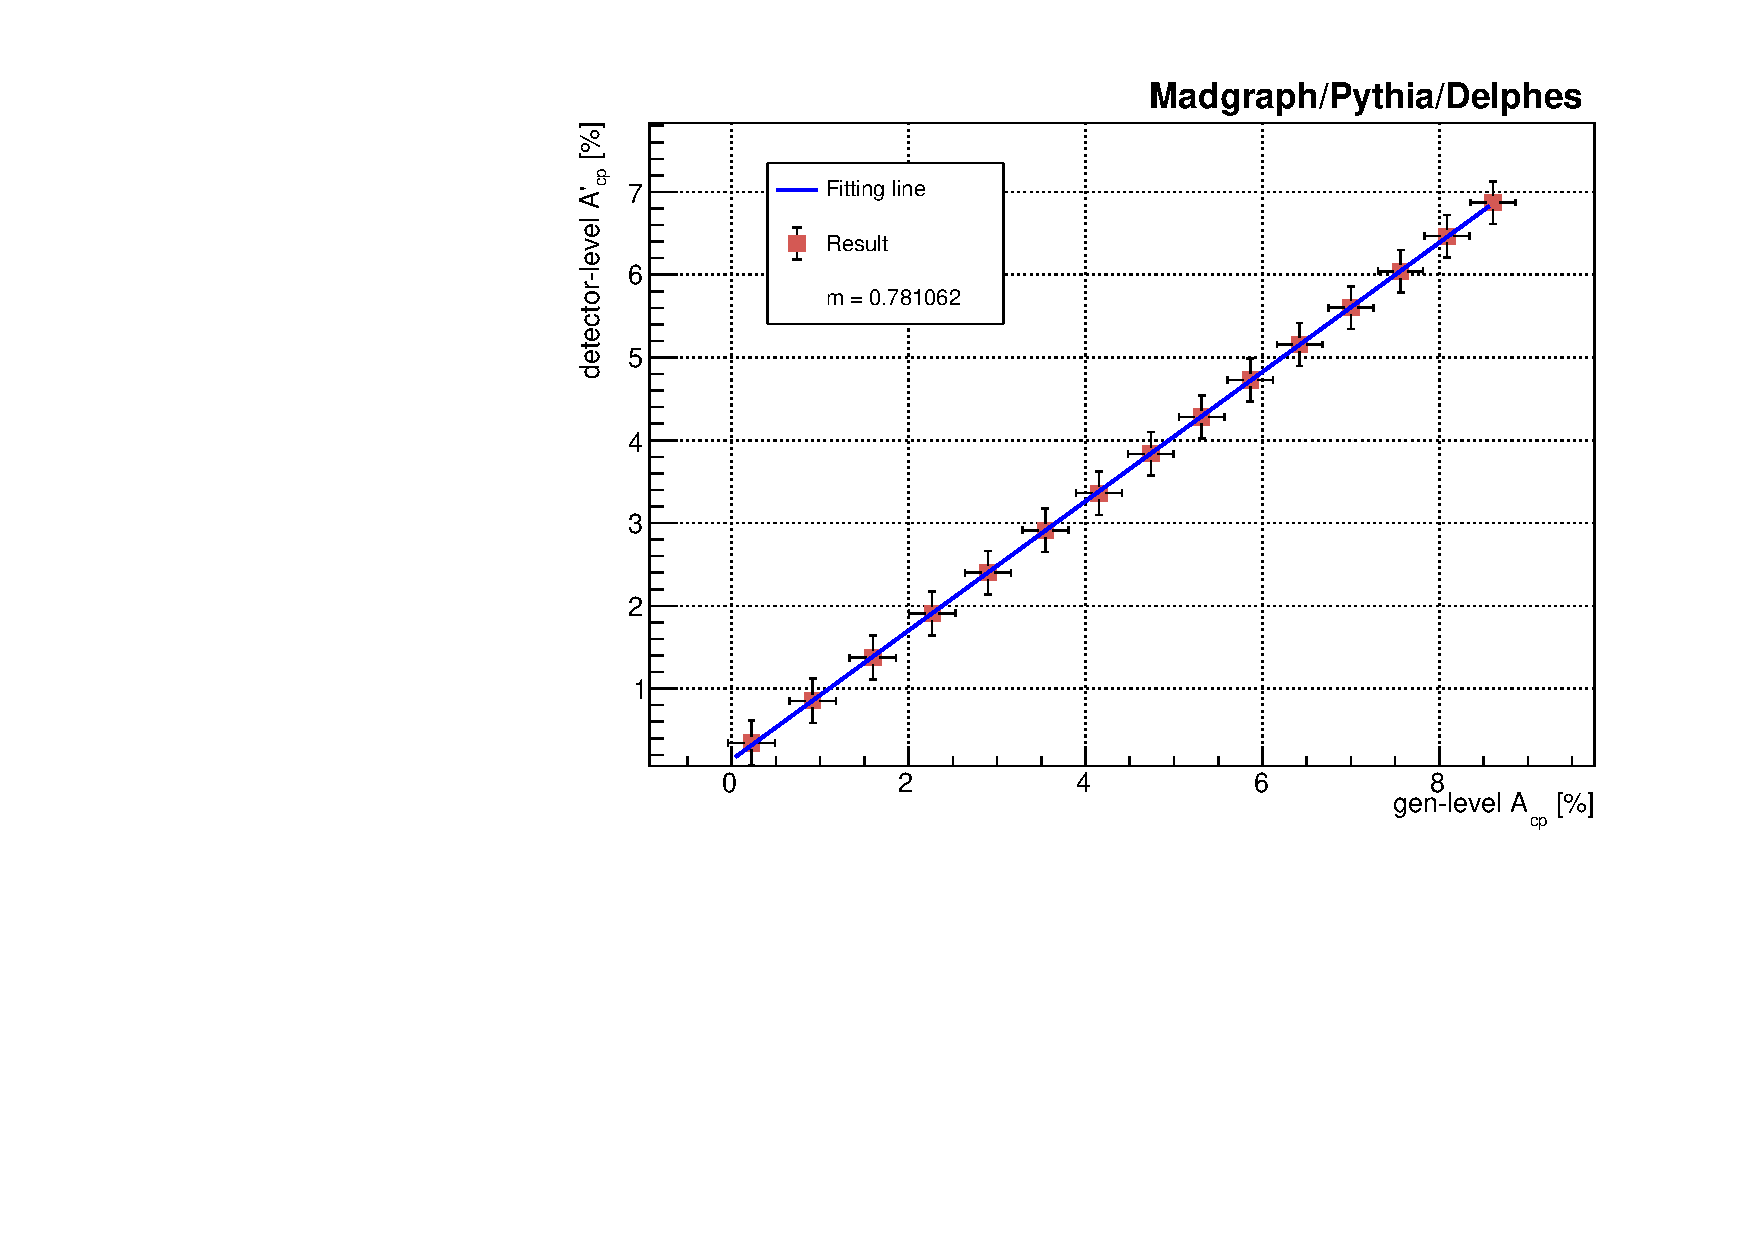
\includegraphics[width=0.45\textwidth]{Figures/Observables/property/text_Dilution_Obs_2HDM_NLO_v1_dr.pdf}}\\
			\caption{Validation of measurred dilution factor with artificial $A_{cp}$'s $t\bar{t}$ simulation samples(2HDM)}
			\label{Obs:fig:vali_2HDM}
			\end{figure}
			\FloatBarrier



\FloatBarrier
